\documentclass[11pt,a4paper]{article}

\usepackage{iftex}

\ifpdftex
  \usepackage[utf8]{vietnam}
  \usepackage{tgpagella}
  \usepackage{amsmath, amssymb}
\else
  \usepackage{fontspec}
  \usepackage{unicode-math}
  \setmainfont{texgyrepagella-regular.otf}[
      BoldFont = texgyrepagella-bold.otf,
      ItalicFont = texgyrepagella-italic.otf,
      BoldItalicFont = texgyrepagella-bolditalic.otf
  ]
  \setmathfont{texgyrepagella-math.otf}
  \usepackage{amsmath}
\fi

\usepackage[a4paper, margin=2.5cm]{geometry}
\usepackage{microtype}
\usepackage{titlesec}
\usepackage{enumitem}
\usepackage{multicol}
\usepackage{graphicx}
\usepackage{tikz}
\usetikzlibrary{arrows.meta}

% Căn chỉnh khoảng cách theo chuẩn học thuật
\linespread{1.05}
\setlength{\parindent}{0pt}
\setlength{\parskip}{5pt plus 2pt minus 1pt}

% Khoảng cách phương trình toán học
\setlength{\abovedisplayskip}{5pt plus 2pt minus 2pt}
\setlength{\belowdisplayskip}{5pt plus 2pt minus 2pt}
\setlength{\abovedisplayshortskip}{3pt plus 1pt}
\setlength{\belowdisplayshortskip}{3pt plus 1pt}

% Định dạng tiêu đề chương
\titleformat{\section}
  {\large\bfseries}
  {\thesection}{0.5em}{}
\titlespacing*{\section}
  {0pt}{14pt plus 3pt minus 2pt}{6pt plus 1pt minus 1pt}

\pagestyle{plain}

\begin{document}

\begin{center}
    {\Large\bfseries LỜI GIẢI CHI TIẾT BÀI TẬP VẬT LÝ ĐIỆN TỬ}\\[0.2cm]
    {\bfseries HỌC PHẦN: PH3330}
\end{center}
\vspace{0.2cm}

%=====================================================================
% CHƯƠNG I
%=====================================================================
\section*{Chương I. Chuyển động của hạt tích điện trong chân không}

\textbf{Bài 1-1.} Tìm biểu thức và xác định độ nhạy của một ống tia điện tử của máy dao động ký có các thông số sau: Hiệu điện thế tăng tốc chùm điện tử là $900\text{ V}$, khoảng cách từ điểm giữa bản lái tia đến màn huỳnh quang bằng $20\text{ cm}$, chiều dài các bản lái tia bằng $2\text{ cm}$, khoảng cách giữa hai bản lái tia bằng $0{,}5\text{ cm}$.

\textbf{Giải.}

\textbf{Dữ kiện:} $U_0 = 900\text{ V}$, $l_1 = 2\text{ cm} = 0{,}02\text{ m}$, $L = \dfrac{l_1}{2} + l_2 = 20\text{ cm} = 0{,}2\text{ m}$, $d = 0{,}5\text{ cm} = 5 \cdot 10^{-3}\text{ m}$. Cần tìm: $S$.

\begin{center}
  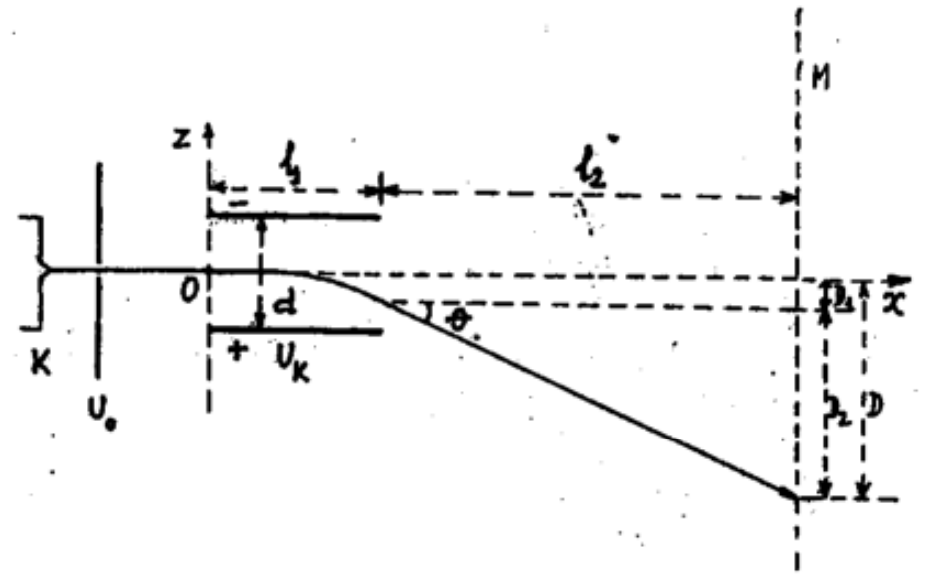
\includegraphics[width=0.62\textwidth]{images/fig_1_1_crt.png}\\[0.1cm]
  \textit{Hình 1.1: Quỹ đạo làm lệch của chùm điện tử qua hai bản lái tia.}
\end{center}

\textbf{B1:} Thiết lập CT tính độ lệch của chùm điện tử trên màn:
\begin{itemize}[leftmargin=*, topsep=1pt, itemsep=1pt]
  \item Vận tốc ban đầu của electron khi ra khỏi anot sau khi được tăng tốc bởi hiệu điện thế $U_0$:
  \begin{equation*}
      \frac{1}{2} m v_0^2 = e U_0 \implies v_0 = \sqrt{\frac{2 e U_0}{m}}
  \end{equation*}
  \item Khi qua bản lái tia dài $l_1$ dưới điện thế lệch $U_K$, cường độ điện trường đều giữa hai bản là $E = \dfrac{U_K}{d}$. Gia tốc theo phương thẳng đứng:
  \begin{equation*}
      a_y = \frac{e E}{m} = \frac{e U_K}{m d}
  \end{equation*}
  \item Thời gian chuyển động trong bản lái tia: $t_1 = \dfrac{l_1}{v_0}$. Độ lệch thẳng đứng và vận tốc thẳng đứng tại mép ra của bản lái tia:
  \begin{equation*}
      y_1 = \frac{1}{2} a_y t_1^2 = \frac{e U_K l_1^2}{2 m d v_0^2} = \frac{l_1^2 U_K}{4 d U_0}, \qquad v_y = a_y t_1 = \frac{e U_K l_1}{m d v_0}
  \end{equation*}
  \item Góc lệch chùm tia $\theta$:
  \begin{equation*}
      \tan\theta = \frac{v_y}{v_0} = \frac{e U_K l_1}{m d v_0^2} = \frac{l_1 U_K}{2 d U_0}
  \end{equation*}
  \item Độ lệch tổng cộng $D$ trên màn huỳnh quang đặt cách tâm bản lái tia khoảng $L = \dfrac{l_1}{2} + l_2$:
  \begin{equation*}
      D = y_1 + l_2 \tan\theta = \tan\theta \left(\frac{l_1}{2} + l_2\right) = \frac{l_1 U_K}{2 d U_0}\left(\frac{l_1}{2} + l_2\right)
  \end{equation*}
\end{itemize}

\textbf{B2:} Biểu thức và giá trị độ nhạy tĩnh điện $S$:
\begin{equation*}
    S = \frac{D}{U_K} = \frac{l_1}{2 d U_0}\left(\frac{l_1}{2} + l_2\right)
\end{equation*}
Thay số:
\begin{equation*}
    S = \frac{0{,}02 \times 0{,}2}{2 \times (5 \cdot 10^{-3}) \times 900} = \boldsymbol{4{,}44 \cdot 10^{-4}\text{ m/V}} \approx \boldsymbol{4{,}5 \cdot 10^{-4}\text{ m/V}} = \boldsymbol{0{,}45\text{ mm/V}}
\end{equation*}

\vspace{0.45cm}

\textbf{Bài 1-2.} Tìm biểu thức và xác định độ nhạy của một ống tia điện tử của máy dao động ký có các thông số sau: Hiệu điện thế tăng tốc chùm điện tử là $900\text{ V}$. Khoảng cách giữa tâm của vùng từ trường làm lệch tia điện tử đến màn huỳnh quang bằng $35\text{ cm}$. Hệ thống lái tia gồm hai cuộn dây Helmholtz hình tròn có bán kính $R = 2{,}5\text{ cm}$ đặt cách nhau một khoảng cách $2z = 5\text{ cm}$. Số vòng dây trên mỗi cuộn là $200$ vòng. Kích thước vùng tác dụng của từ trường là $2R$, trong đó từ trường được xem là đều.

\textit{Chú ý:} Cường độ từ trường trong cuộn Helmholtz được tính bởi công thức:
\begin{equation*}
    H = \frac{i}{2}\frac{WR^2}{(R^2+z^2)^{3/2}}
\end{equation*}
Độ từ thẩm của chân không $\mu_0 = 1{,}26 \cdot 10^{-6}\text{ T}\cdot\text{m/A}$; $i$ là dòng điện trong cuộn dây, $W$ là số vòng dây của cả hai cuộn.

\textbf{Giải.}

\textbf{Dữ kiện:} $U_0 = 900\text{ V}$, $R = 2{,}5\text{ cm} = 0{,}025\text{ m}$, khoảng cách $2z = 5\text{ cm} \implies z = 2{,}5\text{ cm} = R$, bề rộng vùng từ trường $l_1 = 2R = 5\text{ cm} = 0{,}05\text{ m}$, khoảng cách từ tâm vùng từ trường đến màn $L = \dfrac{l_1}{2} + l_2 = 35\text{ cm} = 0{,}35\text{ m}$, $W = 2 \times 200 = 400\text{ vòng}$, $\mu_0 = 1{,}26 \cdot 10^{-6}\text{ T}\cdot\text{m/A}$, $e = 1{,}6 \cdot 10^{-19}\text{ C}$, $m = 9{,}1 \cdot 10^{-31}\text{ kg}$. Cần tìm: $S = \dfrac{D}{i}$.

\begin{center}
  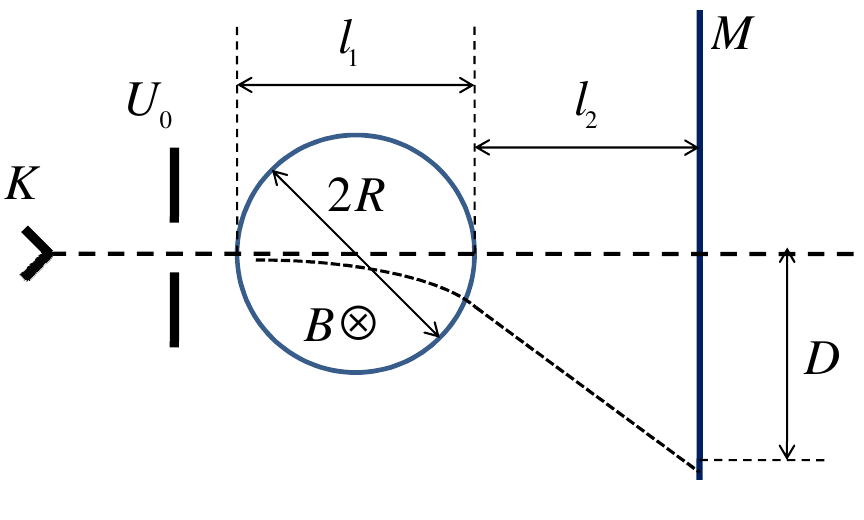
\includegraphics[width=0.55\textwidth]{images/fig_1_2_helmholtz.png}\\[0.1cm]
  \textit{Hình 1.2: Độ lệch của chùm điện tử dưới tác dụng của từ trường cuộn Helmholtz.}
\end{center}

\textbf{B1:} Cảm ứng từ $B$ bên trong hệ cuộn Helmholtz:
\begin{equation*}
    B = \mu_0 H = \frac{\mu_0 i W R^2}{2(R^2+z^2)^{3/2}}
\end{equation*}
Vì $z = R$ nên $(R^2 + z^2)^{3/2} = (2R^2)^{3/2} = 2\sqrt{2}R^3$.

\textbf{B2:} Góc lệch và độ lệch $D$ trên màn:
\begin{itemize}[leftmargin=*, topsep=1pt, itemsep=1pt]
  \item Lực Lorentz đóng vai trò lực hướng tâm: $e v_0 B = \dfrac{m v_0^2}{R_q} \implies R_q = \dfrac{m v_0}{e B}$.
  \item Vì bán kính quỹ đạo $R_q \gg l_1$, góc lệch sau khi qua vùng từ trường:
  \begin{equation*}
      \sin\theta \approx \theta \approx \frac{l_1}{R_q} = \frac{e B l_1}{m v_0} = \frac{e B l_1}{\sqrt{2 m e U_0}} = \sqrt{\frac{e}{2 m U_0}} B l_1
  \end{equation*}
  \item Độ lệch trên màn huỳnh quang:
  \begin{equation*}
      D = \theta \left(\frac{l_1}{2} + l_2\right) = \sqrt{\frac{e}{2 m U_0}} l_1 \left(\frac{l_1}{2} + l_2\right) B
  \end{equation*}
\end{itemize}

\textbf{B3:} Độ nhạy từ trường $S$:
\begin{equation*}
    S = \frac{D}{i} = \sqrt{\frac{e}{2 m U_0}} l_1 \left(\frac{l_1}{2} + l_2\right) \frac{\mu_0 W R^2}{2(R^2+z^2)^{3/2}}
\end{equation*}
Thay số:
\begin{align*}
    \sqrt{\frac{e}{2 m U_0}} &= \sqrt{\frac{1{,}6 \cdot 10^{-19}}{2 \times 9{,}1 \cdot 10^{-31} \times 900}} \approx 9{,}88 \cdot 10^3\text{ C}^{1/2}\text{kg}^{-1/2}\text{V}^{-1/2} \\
    B/i &= \frac{1{,}26 \cdot 10^{-6} \times 400 \times (0{,}025)^2}{2 \times [2 \times (0{,}025)^2]^{3/2}} \approx 3{,}56 \cdot 10^{-3}\text{ T/A} \\
    S &= 9{,}88 \cdot 10^3 \times 0{,}05 \times 0{,}35 \times 3{,}56 \cdot 10^{-3} \approx \boldsymbol{0{,}618\text{ m/A}} = \boldsymbol{618\text{ mm/A}}
\end{align*}

\vspace{0.45cm}

\textbf{Bài 1-3.} Trên đường đi của chùm điện tử người ta đặt một hệ gồm hai lưới có dạng mặt cầu đồng tâm bán kính trung bình là $R = 3\text{ cm}$. Điện thế lưới ngoài là $U_1 = 300\text{ V}$, điện thế lưới trong là $U_2 = 500\text{ V}$ (so với catot phát xạ điện tử). Chứng minh rằng hệ hai lưới này có tính hội tụ đối với chùm điện tử. Tính tiêu cự của hệ.

\textbf{Giải.}

\textbf{Dữ kiện:} $R = 3\text{ cm} = 0{,}03\text{ m}$, $U_1 = 300\text{ V}$, $U_2 = 500\text{ V}$. Cần tìm: $f$.

\begin{center}
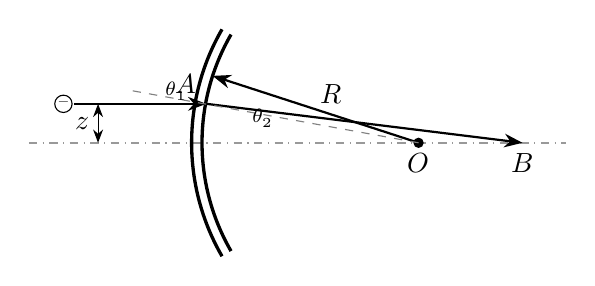
\begin{tikzpicture}[scale=1.1, >=Stealth]
  \draw[dashdotted, thick, gray!80] (-3,0) -- (3.2,0);
  \filldraw (1.5,0) circle (1.5pt) node[below] {$O$};
  \draw[very thick] ([shift=(150:2.5)] 1.5,0) arc (150:210:2.5);
  \draw[very thick] ([shift=(150:2.62)] 1.5,0) arc (150:210:2.62);
  \draw[->, thick] (1.5,0) -- ++(162:2.5) node[midway, above right=-2pt] {$R$};
  \draw (-2.6, 0.45) circle (0.1) node {\tiny $-$};
  \draw[->, thick] (-2.48, 0.45) -- (-0.95, 0.45) node[above left] {$A$};
  \draw[->, thick] (-0.95, 0.45) -- (2.7, 0) node[below] {$B$};
  \draw[dashed, thin, gray] (1.5,0) -- (-1.8, 0.6);
  \node at (-1.3, 0.6) {\scriptsize $\theta_1$};
  \node at (-0.3, 0.28) {\scriptsize $\theta_2$};
  \draw[<->, thin] (-2.2, 0) -- (-2.2, 0.45) node[midway, left] {$z$};
\end{tikzpicture}\\[0.1cm]
\textit{Hình 1.3: Sơ đồ hệ hai lưới cầu đồng tâm cho bài tập (1-3).}
\end{center}

\textbf{B1:} Chứng minh tính hội tụ:
\begin{itemize}[leftmargin=*, topsep=1pt, itemsep=1pt]
  \item Xét hạt điện tử bay song song với trục quang học, cách trục khoảng $z \ll R$. Tia tới gặp mặt lưới tại điểm $A$. Pháp tuyến tại $A$ đi qua tâm cầu $O$.
  \item Gọi góc tới là $\theta_1$ và góc khúc xạ là $\theta_2$. AD định luật khúc xạ quang học điện tử:
  \begin{equation*}
      \sin\theta_1 \sqrt{U_1} = \sin\theta_2 \sqrt{U_2} \implies \frac{\sin\theta_2}{\sin\theta_1} = \sqrt{\frac{U_1}{U_2}} = k
  \end{equation*}
  \item Vì $z \ll R$ nên góc $\theta_1, \theta_2$ rất nhỏ ($\sin\theta \approx \theta$):
  \begin{equation*}
      \theta_2 \approx k \theta_1 = \sqrt{\frac{U_1}{U_2}} \theta_1
  \end{equation*}
  \item Do $U_2 = 500\text{ V} > U_1 = 300\text{ V}$ nên $k = \sqrt{\dfrac{300}{500}} \approx 0{,}775 < 1 \implies \theta_2 < \theta_1$. Tia khúc xạ bị bẻ lệch về phía pháp tuyến $OA$, tức là lệch về phía trục quang học. Vậy hệ hai lưới cầu có \textbf{tính hội tụ}.
\end{itemize}

\textbf{B2:} Xác định tiêu cự $f$:
\begin{itemize}[leftmargin=*, topsep=1pt, itemsep=1pt]
  \item Góc lệch giữa tia khúc xạ và tia tới là $\varphi = \theta_1 - \theta_2 = (1 - k)\theta_1$.
  \item Từ hình học, cung $AC \approx R \theta_1$. Khoảng cách từ đỉnh lưới $C$ đến giao điểm $B$ của tia khúc xạ với trục quang học:
  \begin{equation*}
      CB \approx \frac{AC}{\varphi} = \frac{R \theta_1}{(1 - k)\theta_1} = \frac{R}{1 - k} = \frac{R}{1 - \sqrt{\dfrac{U_1}{U_2}}}
  \end{equation*}
  \item Biểu thức $CB$ hoàn toàn không phụ thuộc vào $z$ (hay $\theta_1$), chứng tỏ mọi tia song song đều hội tụ tại cùng một tiêu điểm $B$. Do đó:
  \begin{equation*}
      f = CB = \frac{R}{1 - \sqrt{\dfrac{U_1}{U_2}}} = \frac{3\text{ cm}}{1 - \sqrt{\dfrac{300}{500}}} \approx \frac{3}{1 - 0{,}7746} = \boldsymbol{13{,}25\text{ cm}} = \boldsymbol{0{,}1325\text{ m}}
  \end{equation*}
\end{itemize}

\vspace{0.45cm}

\textbf{Bài 1-4.} Một hệ quang học điện tử gồm một catot phẳng $K$, một lưới tăng tốc $G$ có điện thế $U_G$ bằng $200\text{ V}$, một tấm ngăn (diapham) có điện thế $U_D$ và một anot $A$ được nối với diapham. Xác định điện thế $U_D$ (so với catot) để chùm điện tử song song hội tụ lên anot. Cho biết khoảng cách giữa lưới tăng tốc đến diapham là $0{,}5\text{ cm}$, khoảng cách giữa diapham đến anot là $0{,}8\text{ cm}$.

\textbf{Giải.}

\textbf{Dữ kiện:} $U_G = 200\text{ V}$, $d_1 = 0{,}5\text{ cm} = 5 \cdot 10^{-3}\text{ m}$, $d_2 = 0{,}8\text{ cm} = 8 \cdot 10^{-3}\text{ m}$, $U_A = U_D$. Cần tìm: $U_D$.

\begin{center}
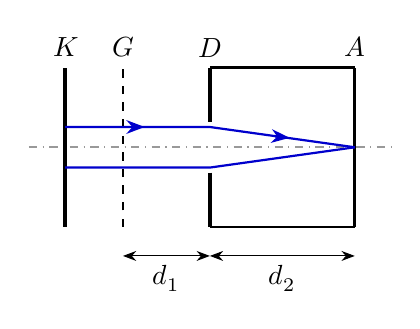
\begin{tikzpicture}[scale=0.92, >=Stealth]
  \draw[dashdotted, thick, gray!80] (-0.5,0) -- (4.5,0);
  \draw[very thick] (0,-1.1) -- (0,1.1) node[above] {$K$};
  \draw[thick, dashed] (0.8,-1.1) -- (0.8,1.1) node[above] {$G$};
  \draw[very thick] (2,0.35) -- (2,1.1);
  \draw[very thick] (2,-0.35) -- (2,-1.1);
  \node[above] at (2,1.1) {$D$};
  \draw[very thick] (4,-1.1) -- (4,1.1) node[above] {$A$};
  \draw[thick] (2,1.1) -- (4,1.1);
  \draw[thick] (2,-1.1) -- (4,-1.1);
  \draw[thick, blue!80!black] (0,0.28) -- (2,0.28) -- (4,0);
  \draw[thick, blue!80!black] (0,-0.28) -- (2,-0.28) -- (4,0);
  \draw[->, thick, blue!80!black] (0.9,0.28) -- (1.1,0.28);
  \draw[->, thick, blue!80!black] (2.9,0.15) -- (3.1,0.13);
  \draw[<->, thin] (0.8,-1.5) -- (2,-1.5) node[midway, below] {$d_1$};
  \draw[<->, thin] (2,-1.5) -- (4,-1.5) node[midway, below] {$d_2$};
\end{tikzpicture}\\[0.1cm]
\textit{Hình 1.4: Sơ đồ hệ quang học điện tử một diapham cho bài tập (1-4).}
\end{center}

\textbf{B1:} AD CT tính tiêu cự thấu kính diapham tròn:
\begin{equation*}
    f = \frac{4 U_D}{E_2 - E_1}
\end{equation*}
Trong đó:
\begin{itemize}[leftmargin=*, topsep=1pt, itemsep=1pt]
  \item Cường độ điện trường trước diapham (vùng $G \to D$): $E_1 = \dfrac{U_D - U_G}{d_1}$.
  \item Cường độ điện trường sau diapham (vùng $D \to A$): Do $U_A = U_D$ nên $E_2 = 0$.
\end{itemize}
Suy ra:
\begin{equation*}
    f = \frac{4 U_D}{0 - \dfrac{U_D - U_G}{d_1}} = \frac{4 U_D d_1}{U_G - U_D}
\end{equation*}

\textbf{B2:} ĐK chùm điện tử song song hội tụ lên anot $A$:
Vì chùm tia tới là chùm song song nên tiêu điểm của thấu kính diapham phải nằm đúng trên bề mặt anot $A$, tức là $f = d_2$:
\begin{equation*}
    \frac{4 U_D d_1}{U_G - U_D} = d_2 \implies 4 d_1 U_D = d_2(U_G - U_D) \implies U_D (4 d_1 + d_2) = d_2 U_G
\end{equation*}
Biểu thức điện thế $U_D$:
\begin{equation*}
    U_D = \frac{d_2}{4 d_1 + d_2} U_G
\end{equation*}
Thay số với $d_1 = 0{,}5\text{ cm}$, $d_2 = 0{,}8\text{ cm}$, $U_G = 200\text{ V}$:
\begin{equation*}
    U_D = \frac{0{,}8}{4 \times 0{,}5 + 0{,}8} \times 200 = \frac{0{,}8}{2{,}8} \times 200 = \boldsymbol{57{,}14\text{ V}} \approx \boldsymbol{57\text{ V}}
\end{equation*}

\vspace{0.45cm}

\textbf{Bài 1-5.} Xét một hệ quang học điện tử gồm một catot $K$, hai diapham $D_1, D_2$ và một anot $A$. Khoảng cách giữa các điện cực đó bằng nhau và bằng $1\text{ cm}$. Điện thế của diapham thứ nhất $D_1$ bằng điện thế anot $A$ và bằng $U_1 = 100\text{ V}$ (so với điện thế catot $K$). Xác định điện thế của diapham thứ hai $D_2$ để cho chùm điện tử song song đi qua hệ hội tụ ở anot $A$.

\textbf{Giải.}

\textbf{Dữ kiện:} $U_K = 0$, $U_{D1} = U_A = U_1 = 100\text{ V}$, $d = 1\text{ cm} = 0{,}01\text{ m}$. Cần tìm: $U_2 = U_{D2}$.

\begin{center}
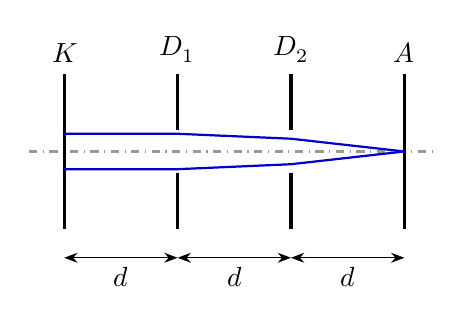
\begin{tikzpicture}[scale=0.9, >=Stealth]
  \draw[dashdotted, thick, gray!80] (-0.5,0) -- (5.2,0);
  \draw[very thick] (0,-1.1) -- (0,1.1) node[above] {$K$};
  \draw[very thick] (1.6,0.3) -- (1.6,1.1) node[above] {$D_1$};
  \draw[very thick] (1.6,-0.3) -- (1.6,-1.1);
  \draw[very thick] (3.2,0.3) -- (3.2,1.1) node[above] {$D_2$};
  \draw[very thick] (3.2,-0.3) -- (3.2,-1.1);
  \draw[very thick] (4.8,-1.1) -- (4.8,1.1) node[above] {$A$};
  \draw[thick, blue!80!black] (0,0.25) -- (1.6,0.25) -- (3.2,0.18) -- (4.8,0);
  \draw[thick, blue!80!black] (0,-0.25) -- (1.6,-0.25) -- (3.2,-0.18) -- (4.8,0);
  \draw[<->, thin] (0,-1.5) -- (1.6,-1.5) node[midway, below] {$d$};
  \draw[<->, thin] (1.6,-1.5) -- (3.2,-1.5) node[midway, below] {$d$};
  \draw[<->, thin] (3.2,-1.5) -- (4.8,-1.5) node[midway, below] {$d$};
\end{tikzpicture}\\[0.1cm]
\textit{Hình 1.5: Sơ đồ hệ quang học điện tử hai diapham cho bài tập (1-5).}
\end{center}

\textbf{B1:} Xác định tiêu cự của hai thấu kính diapham:
\begin{itemize}[leftmargin=*, topsep=1pt, itemsep=1pt]
  \item Tại $D_1$: Cường độ điện trường trước $D_1$ là $E_1 = \dfrac{U_1 - 0}{d} = \dfrac{U_1}{d}$; sau $D_1$ là $E_2 = \dfrac{U_2 - U_1}{d}$.
  \begin{equation*}
      f_1 = \frac{4 U_1}{E_2 - E_1} = \frac{4 U_1}{\dfrac{U_2 - U_1}{d} - \dfrac{U_1}{d}} = \frac{4 U_1 d}{U_2 - 2 U_1}
  \end{equation*}
  \item Tại $D_2$: Cường độ điện trường trước $D_2$ là $E_2 = \dfrac{U_2 - U_1}{d}$; sau $D_2$ là $E_3 = \dfrac{U_1 - U_2}{d} = -E_2$.
  \begin{equation*}
      f_2 = \frac{4 U_2}{E_3 - E_2} = \frac{4 U_2}{-\dfrac{2(U_2 - U_1)}{d}} = -\frac{2 U_2 d}{U_2 - U_1}
  \end{equation*}
\end{itemize}

\textbf{B2:} Áp dụng công thức hệ hai thấu kính đồng trục:
\begin{itemize}[leftmargin=*, topsep=1pt, itemsep=1pt]
  \item Chùm tia tới song song đi qua $D_1$ tạo ảnh tại tiêu điểm của $D_1$, cách $D_1$ khoảng $f_1$. Khoảng cách từ ảnh này tới $D_2$ là $a_2 = d - f_1$.
  \item Chùm tia tiếp tục qua $D_2$ hội tụ trên anot $A$ cách $D_2$ một khoảng $b_2 = d$.
  \item AD công thức thấu kính $\dfrac{1}{a_2} + \dfrac{1}{b_2} = \dfrac{1}{f_2}$:
  \begin{equation*}
      \frac{1}{d - f_1} + \frac{1}{d} = \frac{1}{f_2} \implies \frac{1}{d - f_1} = \frac{1}{f_2} - \frac{1}{d} = \frac{d - f_2}{d f_2}
  \end{equation*}
  \begin{equation*}
      \implies d - f_1 = \frac{d f_2}{d - f_2} \implies f_1 = d - \frac{d f_2}{d - f_2} = \frac{d^2 - 2 d f_2}{d - f_2}
  \end{equation*}
\end{itemize}

\textbf{B3:} Thay $f_1, f_2$ vào giải PT tìm $U_2$:
Thay $f_1 = \dfrac{4 U_1 d}{U_2 - 2 U_1}$ và $f_2 = -\dfrac{2 U_2 d}{U_2 - U_1}$ vào hệ thức trên, rút gọn ta thu được phương trình bậc 2 đối với $U_2$:
\begin{equation*}
    U_2^2 - 460 U_2 + 12000 = 0
\end{equation*}
Giải PT bậc 2 ta được 2 nghiệm thỏa mãn:
\begin{equation*}
    U_2^{(1)} \approx \boldsymbol{432{,}28\text{ V}} \approx \boldsymbol{432\text{ V}}, \qquad U_2^{(2)} \approx \boldsymbol{27{,}72\text{ V}} \approx \boldsymbol{28\text{ V}}
\end{equation*}

\vspace{0.5cm}

%=====================================================================
% CHƯƠNG II
%=====================================================================
\section*{Chương II. Một số vấn đề vật lý lượng tử}

\textbf{Bài 2-1.} Một mặt bằng kali ở cách ngọn đèn $100\text{ W}$ là $75\text{ cm}$. Giả thiết năng lượng bức xạ của đèn trong đơn vị thời gian chỉ bằng $5\%$ công suất định mức. Nếu coi mỗi nguyên tử kali có dạng một đĩa dẹt đường kính $1\text{ \AA}$, hãy xác định thời gian cần thiết để mỗi nguyên tử đó hấp thụ một năng lượng bằng công thoát của nó $\varphi_K \cong 2\text{ eV}$, theo mẫu sóng ánh sáng. Rút ra nhận xét.

\textbf{Giải.}

\textbf{Dữ kiện:} $P = 100\text{ W}$, $P_b = 5\% P = 5\text{ W}$, $R = 75\text{ cm} = 0{,}75\text{ m}$, $d = 1\text{ \AA} = 10^{-10}\text{ m}$, $\varphi_K = 2\text{ eV} = 3{,}2 \cdot 10^{-19}\text{ J}$ (hoặc $\varphi_K = 2{,}2\text{ eV} = 3{,}52 \cdot 10^{-19}\text{ J}$). Cần tìm: $t$.

\begin{center}
  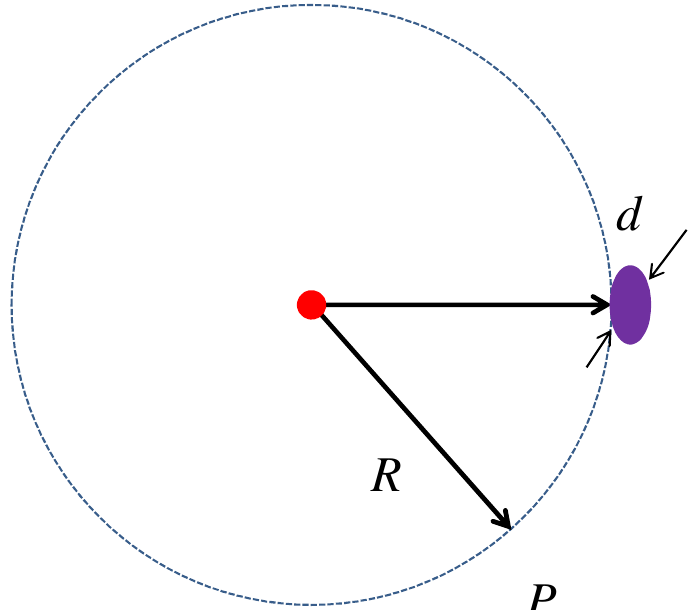
\includegraphics[width=0.38\textwidth]{images/fig_2_1_potassium.png}\\[0.1cm]
  \textit{Hình 2.1: Mô hình bức xạ cầu từ nguồn sáng đến đĩa dẹt nguyên tử Kali.}
\end{center}

\textbf{B1:} Cường độ bức xạ ánh sáng tại vị trí đặt tấm Kali cách nguồn sáng khoảng $R$:
\begin{equation*}
    I = \frac{P_b}{4\pi R^2}
\end{equation*}

\textbf{B2:} Công suất ánh sáng một nguyên tử Kali hấp thụ:
Coi nguyên tử Kali là một đĩa tròn diện tích $S_a = \pi \left(\dfrac{d}{2}\right)^2$:
\begin{equation*}
    P_a = I \cdot S_a = \frac{P_b}{4\pi R^2} \cdot \pi \left(\frac{d}{2}\right)^2 = \frac{P_b d^2}{16 R^2}
\end{equation*}

\textbf{B3:} Thời gian cần thiết để hấp thụ năng lượng bằng công thoát $\varphi_K$:
\begin{equation*}
    t = \frac{\varphi_K}{P_a} = \frac{16 R^2 \varphi_K}{P_b d^2}
\end{equation*}
Thay số với $\varphi_K = 2{,}2\text{ eV} = 2{,}2 \times 1{,}6 \cdot 10^{-19}\text{ J}$:
\begin{equation*}
    t = \frac{16 \times (0{,}75)^2 \times (2{,}2 \times 1{,}6 \cdot 10^{-19})}{5 \times (10^{-10})^2} \approx \boldsymbol{57{,}6\text{ s}}
\end{equation*}
(Nếu lấy $\varphi_K = 2\text{ eV}$ thì $t = \boldsymbol{52{,}4\text{ s}}$).

\textbf{Nhận xét:} Theo quan điểm sóng cổ điển, thời gian tích lũy năng lượng kéo dài tới gần 1 phút. Tuy nhiên, thực nghiệm quang điện chứng minh electron phát ra tức thời ($\sim 10^{-9}\text{ s}$). Mẫu sóng cổ điển không thể giải thích được hiện tượng quang điện, đòi hỏi thuyết lượng tử photon của Einstein.

\vspace{0.45cm}

\textbf{Bài 2-2.} Người ta chiếu kali bằng tia cực tím bước sóng $2500\text{ \AA}$. Biết công thoát của kali là $2{,}2\text{ eV}$, tính động năng cực đại của các electron phát ra. Nếu cường độ bức xạ tới là $2\text{ W/m}^2$, tính số điện tử do một đơn vị diện tích phát ra trong một đơn vị thời gian.

\textbf{Giải.}

\textbf{Dữ kiện:} $\lambda = 2500\text{ \AA} = 2{,}5 \cdot 10^{-7}\text{ m}$, $\varphi_K = 2{,}2\text{ eV}$, $I = 2\text{ W/m}^2$. Cần tìm: $T_{\max}$, $J_e$.

\textbf{B1:} AD PT Einstein cho hiện tượng quang điện, tính động năng cực đại:
\begin{equation*}
    T_{\max} = \frac{h c}{\lambda} - \varphi_K = \frac{6{,}626 \cdot 10^{-34} \times 3 \cdot 10^8}{2{,}5 \cdot 10^{-7} \times 1{,}6 \cdot 10^{-19}} - 2{,}2 = 4{,}969\text{ eV} - 2{,}2\text{ eV} = \boldsymbol{2{,}77\text{ eV}} \approx \boldsymbol{2{,}75\text{ eV}}
\end{equation*}
Đổi ra Jun: $T_{\max} \approx \boldsymbol{4{,}43 \cdot 10^{-19}\text{ J}}$.

\textbf{B2:} Số photon đập vào $1\text{ m}^2$ bề mặt Kali trong $1\text{ s}$:
\begin{equation*}
    N_{ph} = \frac{I}{E_{ph}} = \frac{I \lambda}{h c} = \frac{2 \times 2{,}5 \cdot 10^{-7}}{6{,}626 \cdot 10^{-34} \times 3 \cdot 10^8} \approx 2{,}515 \cdot 10^{18}\text{ photon}/(\text{m}^2\cdot\text{s})
\end{equation*}
Giả sử hiệu suất lượng tử $100\%$ (mỗi photon hấp thụ bứt ra 1 electron), mật độ dòng hạt electron phát xạ:
\begin{equation*}
    J_e = N_e = N_{ph} \approx \boldsymbol{2{,}52 \cdot 10^{18}\text{ e}/(\text{m}^2\cdot\text{s})}
\end{equation*}

\vspace{0.45cm}

\textbf{Bài 2-3.} Một photon có năng lượng $0{,}3\text{ MeV}$ va chạm với một electron đứng yên và tán xạ ngược ($180^\circ$). Xác định vận tốc của electron giật lùi.

\textbf{Giải.}

\textbf{Dữ kiện:} $E_{ph} = 0{,}3\text{ MeV}$, góc tán xạ $\theta = 180^\circ$, năng lượng nghỉ electron $E_0 = m_0 c^2 = 0{,}511\text{ MeV}$. Cần tìm: $v$.

\begin{center}
  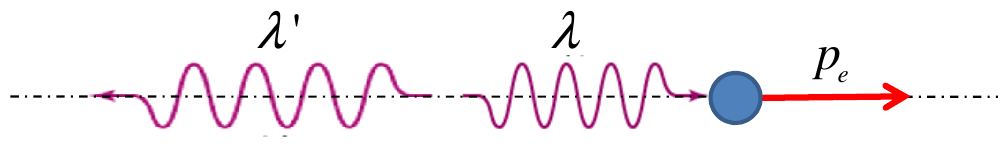
\includegraphics[width=0.68\textwidth]{images/fig_2_3_compton.png}\\[0.1cm]
  \textit{Hình 2.2: Sơ đồ va chạm tán xạ Compton ngược ($180^\circ$).}
\end{center}

\textbf{B1:} AD định luật bảo toàn năng lượng và động lượng (tán xạ ngược $\theta = 180^\circ$):
\begin{itemize}[leftmargin=*, topsep=1pt, itemsep=1pt]
  \item Bảo toàn năng lượng: $E_{ph} + E_0 = E_{ph}' + E_e = \dfrac{h c}{\lambda'} + m_e c^2$.
  \item Bảo toàn động lượng: $\dfrac{h}{\lambda} = -\dfrac{h}{\lambda'} + p_e \implies \dfrac{h c}{\lambda} = -\dfrac{h c}{\lambda'} + p_e c$.
  \item Cộng hai vế hai phương trình:
  \begin{equation*}
      2 E_{ph} + E_0 = m_e c^2 + p_e c = m_0 \gamma c^2 + m_0 \gamma v c = E_0 \gamma \left(1 + \frac{v}{c}\right)
  \end{equation*}
  với $\gamma = \dfrac{1}{\sqrt{1 - v^2/c^2}}$. Do đó:
  \begin{equation*}
      \left(\frac{2 E_{ph} + E_0}{E_0}\right)^2 = \gamma^2 \left(1 + \frac{v}{c}\right)^2 = \frac{(1 + v/c)^2}{1 - v^2/c^2} = \frac{1 + v/c}{1 - v/c}
  \end{equation*}
\end{itemize}

\textbf{B2:} Đặt $\alpha = \left(\dfrac{2 E_{ph} + E_0}{E_0}\right)^2 = \left(\dfrac{2 \times 0{,}3}{0{,}511} + 1\right)^2 \approx (2{,}174)^2 \approx 4{,}727$:
\begin{equation*}
    \frac{1 + v/c}{1 - v/c} = \alpha \implies \frac{v}{c} = \frac{\alpha - 1}{\alpha + 1} = \frac{4{,}727 - 1}{4{,}727 + 1} \approx \boldsymbol{0{,}65}
\end{equation*}
Vận tốc của electron giật lùi:
\begin{equation*}
    v = 0{,}65 c \approx \boldsymbol{1{,}95 \cdot 10^8\text{ m/s}}
\end{equation*}

\vspace{0.45cm}

\textbf{Bài 2-4.} Tìm hiệu điện thế $U$ cần thiết để electron có bước sóng de Broglie bằng $1\text{ \AA}$.

\textbf{Giải.}

\textbf{Dữ kiện:} $\lambda = 1\text{ \AA} = 10^{-10}\text{ m}$. Cần tìm: $U$.

\textbf{B1:} Bước sóng de Broglie của electron phi tương đối tính qua hiệu điện thế gia tốc $U$:
\begin{equation*}
    \lambda = \frac{h}{p} = \frac{h}{\sqrt{2 m e U}} \implies \lambda = \frac{12{,}27}{\sqrt{U\text{ (V)}}}\text{ \AA}
\end{equation*}

\textbf{B2:} Tính $U$:
\begin{equation*}
    U = \left(\frac{12{,}27}{\lambda\text{ (\AA)}}\right)^2 = \left(\frac{12{,}27}{1}\right)^2 \approx \boldsymbol{151\text{ V}}
\end{equation*}

\vspace{0.45cm}

\textbf{Bài 2-5.} Hãy chứng minh rằng bước sóng de Broglie của một hạt tương đối tính có động năng rất lớn so với năng lượng nghỉ của nó ($E \gg E_0$) sẽ bằng bước sóng của photon có cùng năng lượng.

\textbf{Giải.}

\textbf{B1:} Năng lượng toàn phần của hạt tương đối tính:
\begin{equation*}
    E = \sqrt{p^2 c^2 + E_0^2}
\end{equation*}
Khi $E \gg E_0$ (trường hợp siêu tương đối tính): $E \approx p c \implies p \approx \dfrac{E}{c}$.

\textbf{B2:} Bước sóng de Broglie của hạt:
\begin{equation*}
    \lambda_{\text{hạt}} = \frac{h}{p} \approx \frac{h c}{E}
\end{equation*}
Đối với photon có năng lượng $E$, bước sóng ánh sáng là:
\begin{equation*}
    \lambda_{\text{photon}} = \frac{h c}{E}
\end{equation*}
Như vậy: $\lambda_{\text{hạt}} \approx \lambda_{\text{photon}} = \boldsymbol{\dfrac{h c}{E}}$ (đpcm).

\vspace{0.45cm}

\textbf{Bài 2-6.} Hãy tìm mối liên hệ giữa vận tốc pha $v_f$ và vận tốc nhóm $v_g$ của sóng de Broglie đối với một hạt tự do có vận tốc $v$.

\textbf{Giải.}

\textbf{B1:} Vận tốc pha $v_f$:
\begin{equation*}
    v_f = \frac{\omega}{k} = \frac{E}{p} = \frac{m c^2}{m v} = \boldsymbol{\frac{c^2}{v}}
\end{equation*}
(Vì $v < c$ nên $v_f > c$, vận tốc pha của sóng de Broglie lớn hơn vận tốc ánh sáng nhưng không mang năng lượng).

\textbf{B2:} Vận tốc nhóm $v_g$:
Từ hệ thức Einstein: $E^2 = p^2 c^2 + m_0^2 c^4$. Lấy vi phân hai vế:
\begin{equation*}
    2 E \, dE = 2 p c^2 \, dp \implies \frac{dE}{dp} = \frac{p c^2}{E}
\end{equation*}
Vận tốc nhóm của gói sóng de Broglie:
\begin{equation*}
    v_g = \frac{d\omega}{dk} = \frac{dE}{dp} = \frac{(m v) c^2}{m c^2} = \boldsymbol{v}
\end{equation*}
(Vận tốc nhóm trùng với vận tốc chuyển động thực của hạt). Ta cũng có hệ thức: $v_f \cdot v_g = c^2$.

\vspace{0.45cm}

\textbf{Bài 2-8.} Trong một thí nghiệm giao thoa khe Young cho chùm hạt có thông số: $h = 6{,}625 \cdot 10^{-3}\text{ J}\cdot\text{s}$, $m = 66{,}25 \cdot 10^{-3}\text{ kg}$, vận tốc hạt $v = 5\text{ m/s}$, khoảng cách giữa hai khe $d = 0{,}6\text{ m}$, khoảng cách từ khe tới màn $L = 12\text{ m}$. Tính khoảng vân giao thoa $\Delta y$.

\textbf{Giải.}

\textbf{Dữ kiện:} $h = 6{,}625 \cdot 10^{-3}\text{ J}\cdot\text{s}$, $m = 66{,}25 \cdot 10^{-3}\text{ kg}$, $v = 5\text{ m/s}$, $d = 0{,}6\text{ m}$, $L = 12\text{ m}$. Cần tìm: $\Delta y$.

\begin{center}
  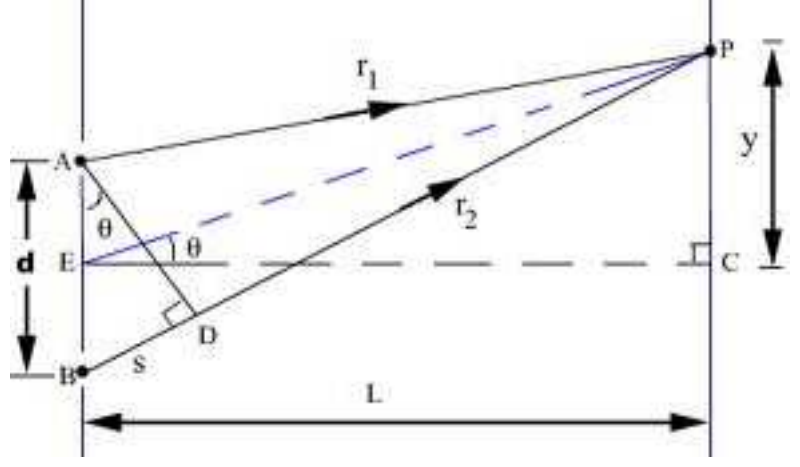
\includegraphics[width=0.52\textwidth]{images/fig_2_8_doubleslit.png}\\[0.1cm]
  \textit{Hình 2.3: Giao thoa sóng vật chất qua hai khe hẹp.}
\end{center}

\textbf{B1:} Bước sóng de Broglie của chùm hạt:
\begin{equation*}
    \lambda = \frac{h}{p} = \frac{h}{m v}
\end{equation*}

\textbf{B2:} Khoảng vân giao thoa $\Delta y$:
\begin{equation*}
    \Delta y = \frac{\lambda L}{d} = \frac{h L}{m v d} = \frac{6{,}625 \cdot 10^{-3} \times 12}{66{,}25 \cdot 10^{-3} \times 5 \times 0{,}6} = \boldsymbol{0{,}4\text{ m}}
\end{equation*}

\vspace{0.45cm}

\textbf{Bài 2-9.} Áp dụng hệ thức bất định Heisenberg $\Delta x \cdot \Delta p_x \ge \hbar = \dfrac{h}{2\pi}$. Biết độ bất định tương đối về xung lượng là $\dfrac{\Delta p}{p} = 10^{-3}$. Hãy xác định độ bất định tọa độ $\Delta x$ đối với:
\begin{enumerate}[label=\alph*)]
  \item Một hạt bụi có khối lượng $m = 5\text{ mg}$ chuyển động với vận tốc $v = 2\text{ m/s}$.
  \item Một electron chuyển động với vận tốc $v = 1{,}8 \cdot 10^8\text{ m/s}$.
\end{enumerate}

\textbf{Giải.}

\textbf{B1:} Đối với hạt bụi (vật lý cổ điển):
\begin{itemize}[leftmargin=*, topsep=1pt, itemsep=1pt]
  \item Xung lượng: $p = m v = (5 \cdot 10^{-6}\text{ kg}) \times 2\text{ m/s} = 10^{-5}\text{ kg}\cdot\text{m/s}$.
  \item Độ bất định xung lượng: $\Delta p = 10^{-3} p = 10^{-8}\text{ kg}\cdot\text{m/s}$.
  \item Độ bất định tọa độ:
  \begin{equation*}
      \Delta x \ge \frac{h}{2\pi \Delta p} = \frac{6{,}626 \cdot 10^{-34}}{2\pi \times 10^{-8}} \approx 1{,}055 \cdot 10^{-26}\text{ m} = \boldsymbol{1{,}056 \cdot 10^{-16}\text{ \AA}}
  \end{equation*}
  (Độ bất định tọa độ vô cùng nhỏ so với kích thước hạt bụi, có thể xem hạt chuyển động theo quỹ đạo xác định).
\end{itemize}

\textbf{B2:} Đối với electron ($v = 1{,}8 \cdot 10^8\text{ m/s} = 0{,}6c$):
\begin{itemize}[leftmargin=*, topsep=1pt, itemsep=1pt]
  \item Electron chuyển động tương đối tính:
  \begin{equation*}
      p = \frac{m_0 v}{\sqrt{1 - v^2/c^2}} = \frac{9{,}1 \cdot 10^{-31} \times 1{,}8 \cdot 10^8}{\sqrt{1 - 0{,}6^2}} = \frac{1{,}638 \cdot 10^{-22}}{0{,}8} = 2{,}0475 \cdot 10^{-22}\text{ kg}\cdot\text{m/s}
  \end{equation*}
  \item Độ bất định xung lượng: $\Delta p = 10^{-3} p = 2{,}0475 \cdot 10^{-25}\text{ kg}\cdot\text{m/s}$.
  \item Độ bất định tọa độ:
  \begin{equation*}
      \Delta x \ge \frac{h}{2\pi \Delta p} = \frac{6{,}626 \cdot 10^{-34}}{2\pi \times 2{,}0475 \cdot 10^{-25}} \approx 5{,}15 \cdot 10^{-10}\text{ m} \approx \boldsymbol{5{,}14\text{ \AA}}
  \end{equation*}
  (Độ bất định tọa độ lớn hơn kích thước nguyên tử ($\sim 1\text{ \AA}$), chứng tỏ electron trong thang vi mô không có khái niệm quỹ đạo cổ điển).
\end{itemize}

\vspace{0.45cm}

\textbf{Bài 2-10.} Một nguyên tử bức xạ ánh sáng có bước sóng $\lambda = 2500\text{ \AA}$ với độ rộng vạch $\Delta\lambda = 1\text{ \AA}$. Tính thời gian sống tối thiểu của trạng thái kích thích.

\textbf{Giải.}

\textbf{B1:} AD hệ thức bất định năng lượng -- thời gian:
\begin{equation*}
    \Delta E \cdot \Delta t \ge \frac{h}{2\pi} \implies \Delta t \ge \frac{h}{2\pi \Delta E}
\end{equation*}

\textbf{B2:} Năng lượng photon $E = \dfrac{h c}{\lambda} \implies \Delta E \approx \dfrac{h c}{\lambda^2} \Delta\lambda$. Suy ra:
\begin{equation*}
    \Delta t \ge \frac{h}{2\pi \dfrac{h c}{\lambda^2}\Delta\lambda} = \frac{\lambda^2}{2\pi c \Delta\lambda}
\end{equation*}
Thay số với $\lambda = 2500\text{ \AA} = 2{,}5 \cdot 10^{-7}\text{ m}$ và $\Delta\lambda = 1\text{ \AA} = 10^{-10}\text{ m}$:
\begin{equation*}
    \Delta t \ge \frac{(2{,}5 \cdot 10^{-7})^2}{2\pi \times 3 \cdot 10^8 \times 10^{-10}} \approx \boldsymbol{8{,}49 \cdot 10^{-9}\text{ s}} \approx \boldsymbol{8{,}5\text{ ns}}
\end{equation*}

\vspace{0.45cm}

\textbf{Bài 2-11.} Hãy tìm độ bất định về tọa độ của một hạt nếu độ bất định về xung lượng bằng chính xung lượng của nó ($\Delta p = p$).

\textbf{Giải.}

\textbf{B1:} Xung lượng hạt liên hệ với bước sóng de Broglie: $p = \dfrac{h}{\lambda} \implies \Delta p = \dfrac{h}{\lambda}$.

\textbf{B2:} AD hệ thức bất định Heisenberg $\Delta x \cdot \Delta p \ge \dfrac{h}{2\pi}$:
\begin{equation*}
    \Delta x \ge \frac{h}{2\pi \Delta p} = \frac{h}{2\pi \dfrac{h}{\lambda}} = \boldsymbol{\frac{\lambda}{2\pi}}
\end{equation*}

\vspace{0.45cm}

\textbf{Bài 2-13.} Đánh giá động năng cực tiểu của một hạt khối lượng $m$ bị giam giữ trong một miền không gian có kích thước tuyến tính $L$.

\textbf{Giải.}

\textbf{B1:} Hạt bị giam giữ trong miền có kích thước $L$, độ bất định tọa độ $\Delta x \approx L$. AD hệ thức Heisenberg:
\begin{equation*}
    \Delta p_x \ge \frac{h}{2\pi L}
\end{equation*}

\textbf{B2:} Động năng cực tiểu của hạt:
\begin{equation*}
    T_{\min} \approx \frac{(\Delta p_x)^2}{2m} = \boldsymbol{\frac{h^2}{8\pi^2 m L^2}}
\end{equation*}
(Áp dụng cho nucleon trong hạt nhân kích thước $L \sim 10^{-14}\text{ m}$, ta thu được $T_{\min} \approx \boldsymbol{9{,}35\text{ MeV}}$).

\vspace{0.45cm}

\textbf{Bài 2-15.} Một hạt có khối lượng $m = 10^{-14}\text{ kg}$ chuyển động trong một giếng thế năng một chiều sâu vô hạn có bề rộng $L = 0{,}1\text{ mm}$.
\begin{enumerate}[label=\alph*)]
  \item Tính vận tốc nhỏ nhất của hạt.
  \item Xác định số lượng tử $n$ của mức năng lượng khi hạt chuyển động với vận tốc $v = 10^{-5}\text{ m/s}$.
\end{enumerate}

\textbf{Giải.}

\textbf{Dữ kiện:} $m = 10^{-14}\text{ kg}$, $L = 0{,}1\text{ mm} = 10^{-4}\text{ m}$.

\textbf{B1:} Mức năng lượng của hạt trong giếng thế 1 chiều thành vô hạn:
\begin{equation*}
    E_n = n^2 \frac{h^2}{8 m L^2}
\end{equation*}
Năng lượng nhỏ nhất ứng với trạng thái cơ bản $n = 1$: $E_1 = \dfrac{h^2}{8 m L^2}$.
Vận tốc nhỏ nhất tương ứng:
\begin{equation*}
    v_{\min} = \sqrt{\frac{2 E_1}{m}} = \frac{h}{2 m L} = \frac{6{,}625 \cdot 10^{-34}}{2 \times 10^{-14} \times 10^{-4}} = \boldsymbol{3{,}3 \cdot 10^{-16}\text{ m/s}}
\end{equation*}

\textbf{B2:} Khi hạt có vận tốc $v = 10^{-5}\text{ m/s}$, động năng $E = \dfrac{1}{2} m v^2$:
\begin{equation*}
    n = \sqrt{\frac{E}{E_1}} = \frac{2 m L v}{h} = \frac{2 \times 10^{-14} \times 10^{-4} \times 10^{-5}}{6{,}625 \cdot 10^{-34}} \approx \boldsymbol{3 \cdot 10^{10}}
\end{equation*}
Số lượng tử $n$ vô cùng lớn, chứng tỏ trong thế giới vĩ mô các mức năng lượng san sát nhau tạo thành phổ liên tục (nguyên lý tương ứng Bohr).

\vspace{0.45cm}

\textbf{Bài 2-16.} Chứng minh rằng phổ trị riêng của toán tử hình chiếu xung lượng $\hat{p}_x = -i\hbar \dfrac{d}{dx}$ của hạt tự do là phổ liên tục.

\textbf{Giải.}

\textbf{B1:} Phương trình trị riêng của toán tử xung lượng $\hat{p}_x \Psi(x) = p_x \Psi(x)$:
\begin{equation*}
    -i\hbar \frac{d\Psi}{dx} = p_x \Psi \implies \frac{d\Psi}{\Psi} = \frac{i p_x}{\hbar} dx
\end{equation*}

\textbf{B2:} Lấy tích phân ta được hàm riêng:
\begin{equation*}
    \Psi(x) = C e^{i p_x x / \hbar}
\end{equation*}
Vì hạt chuyển động tự do trên toàn bộ trục $-\infty < x < +\infty$, hàm riêng $\Psi(x)$ liên tục, đơn trị và bị chặn (hữu hạn) với \textbf{mọi giá trị thực} của $p_x$. Do đó, xung lượng của hạt tự do có thể nhận bất kỳ giá trị thực nào, tức là phổ trị riêng của xung lượng hạt tự do là \textbf{phổ liên tục} (không bị lượng tử hóa).

\vspace{0.45cm}

\textbf{Bài 2-17.} Hạt electron có năng lượng $E = 50\text{ eV}$ gặp một hàng rào thế năng chữ nhật cao $U_0 = 70\text{ eV}$. Tính hệ số thẩm thấu đường ngầm $D$ khi bề rộng của hàng rào là: a) $L = 1\text{ nm}$; b) $L = 0{,}1\text{ nm}$.

\textbf{Giải.}

\textbf{Dữ kiện:} $E = 50\text{ eV}$, $U_0 = 70\text{ eV} \implies U_0 - E = 20\text{ eV} = 3{,}2 \cdot 10^{-18}\text{ J}$, $m = 9{,}1 \cdot 10^{-31}\text{ kg}$.

\begin{center}
  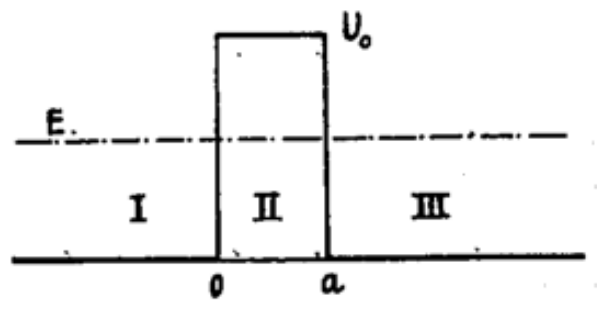
\includegraphics[width=0.48\textwidth]{images/fig_2_17_barrier.png}\\[0.1cm]
  \textit{Hình 2.4: Hiệu ứng đường ngầm xuyên qua hàng rào thế năng chữ nhật ($E < U_0$).}
\end{center}

\textbf{B1:} AD CT tính hệ số thẩm thấu đường ngầm cho hàng rào thế chữ nhật:
\begin{equation*}
    D \approx \exp\left(-\frac{2 L}{\hbar}\sqrt{2 m(U_0 - E)}\right)
\end{equation*}
Số hạng trong hàm mũ:
\begin{equation*}
    \frac{2\sqrt{2 m (U_0 - E)}}{\hbar} = \frac{2 \times \sqrt{2 \times 9{,}1 \cdot 10^{-31} \times 3{,}2 \cdot 10^{-18}}}{1{,}055 \cdot 10^{-34}} \approx 4{,}575 \cdot 10^{10}\text{ m}^{-1}
\end{equation*}

\textbf{B2:} Tính giá trị cho từng trường hợp bề rộng rào:
\begin{enumerate}[label=\alph*)]
  \item Khi $L = 1\text{ nm} = 10^{-9}\text{ m}$:
  \begin{equation*}
      D = e^{-4{,}575 \cdot 10^{10} \times 10^{-9}} = e^{-45{,}75} \approx \boldsymbol{1{,}3 \cdot 10^{-20}}
  \end{equation*}
  (Xác suất xuyên hầm cực kỳ nhỏ, hạt hầu như bị phản xạ hoàn toàn).
  \item Khi $L = 0{,}1\text{ nm} = 10^{-10}\text{ m}$:
  \begin{equation*}
      D = e^{-4{,}575 \cdot 10^{10} \times 10^{-10}} = e^{-4{,}575} \approx \boldsymbol{1{,}03 \cdot 10^{-2}} \approx \boldsymbol{0{,}01} = \boldsymbol{1\%}
  \end{equation*}
  (Khi bề rộng rào mỏng cỡ kích thước nguyên tử, hiệu ứng đường ngầm xuất hiện rõ rệt).
\end{enumerate}

\vspace{0.45cm}

\textbf{Bài 2-18.} Một electron chuyển động trong giếng thế năng 1 chiều sâu vô hạn bề rộng $L = 10^{-10}\text{ m} = 1\text{ \AA}$.
\begin{enumerate}[label=\alph*)]
  \item Chuẩn hóa hàm sóng của electron trong giếng thế: $\Psi_n(x) = A_n \sin\left(\dfrac{n\pi x}{L}\right)$.
  \item Xác định các giá trị năng lượng ở 3 mức thấp nhất ($n = 1, 2, 3$) và bước sóng của photon phát ra khi electron chuyển từ mức $n = 2$ về mức $n = 1$.
\end{enumerate}

\textbf{Giải.}

\begin{center}
  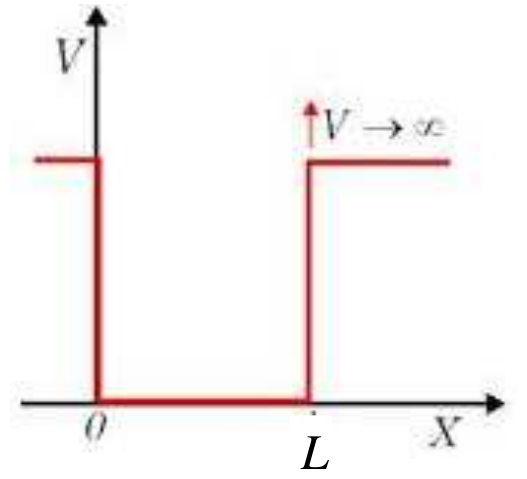
\includegraphics[width=0.36\textwidth]{images/fig_2_18_well.png}\\[0.1cm]
  \textit{Hình 2.5: Giếng thế năng một chiều sâu vô hạn.}
\end{center}

\textbf{B1:} Chuẩn hóa hàm sóng $\Psi_n(x)$:
AD điều kiện chuẩn hóa trên đoạn $[0, L]$:
\begin{equation*}
    \int_0^L |\Psi_n(x)|^2 dx = 1 \implies A_n^2 \int_0^L \sin^2\left(\frac{n\pi x}{L}\right) dx = A_n^2 \int_0^L \frac{1 - \cos\left(\dfrac{2n\pi x}{L}\right)}{2} dx = A_n^2 \frac{L}{2} = 1
\end{equation*}
\begin{equation*}
    \implies A_n = \boldsymbol{\sqrt{\frac{2}{L}}}
\end{equation*}

\textbf{B2:} Năng lượng ở 3 mức đầu tiên ($E_n = n^2 E_1$):
\begin{equation*}
    E_1 = \frac{h^2}{8 m L^2} = \frac{(6{,}625 \cdot 10^{-34})^2}{8 \times 9{,}1 \cdot 10^{-31} \times (10^{-10})^2} \approx 6{,}03 \cdot 10^{-18}\text{ J} = \boldsymbol{37{,}7\text{ eV}}
\end{equation*}
\begin{equation*}
    E_2 = 2^2 E_1 = 4 \times 37{,}7\text{ eV} = \boldsymbol{151\text{ eV}}, \qquad E_3 = 3^2 E_1 = 9 \times 37{,}7\text{ eV} = \boldsymbol{339\text{ eV}}
\end{equation*}

\textbf{B3:} Bước sóng photon phát ra khi chuyển từ mức $n = 2$ về $n = 1$:
\begin{equation*}
    \Delta E = E_2 - E_1 = 151\text{ eV} - 37{,}7\text{ eV} = 113{,}3\text{ eV} = 113{,}3 \times 1{,}6 \cdot 10^{-19}\text{ J} \approx 1{,}813 \cdot 10^{-17}\text{ J}
\end{equation*}
\begin{equation*}
    \lambda = \frac{h c}{\Delta E} = \frac{6{,}625 \cdot 10^{-34} \times 3 \cdot 10^8}{1{,}813 \cdot 10^{-17}} \approx \boldsymbol{1{,}1 \cdot 10^{-8}\text{ m}} = \boldsymbol{11\text{ nm}}
\end{equation*}

\vspace{0.5cm}

%=====================================================================
% CHƯƠNG III
%=====================================================================
\section*{Chương III. Cấu trúc nguyên tử và quang phổ nguyên tử}

\textbf{Bài 3-1.} Tính bước sóng ngắn nhất và bước sóng dài nhất (bằng $\text{\AA}$) đối với dãy Lyman của nguyên tử hydro.

\textbf{Giải.}

\textbf{Dữ kiện:} Dãy Lyman tương ứng $n_1 = 1$, hằng số Rydberg $R \approx 1{,}097 \cdot 10^7\text{ m}^{-1} = 1{,}097 \cdot 10^{-3}\text{ \AA}^{-1}$.

\textbf{B1:} AD công thức Rydberg cho dãy Lyman:
\begin{equation*}
    \frac{1}{\lambda} = R \left(\frac{1}{1^2} - \frac{1}{n_2^2}\right), \qquad (n_2 = 2, 3, 4, \dots)
\end{equation*}

\textbf{B2:} Tính bước sóng:
\begin{itemize}[leftmargin=*, topsep=1pt, itemsep=1pt]
  \item Bước sóng dài nhất ứng với $n_2 = 2$:
  \begin{equation*}
      \frac{1}{\lambda_{\max}} = R\left(1 - \frac{1}{4}\right) = \frac{3R}{4} \implies \lambda_{\max} = \frac{4}{3R} = \frac{4}{3 \times 1{,}097 \cdot 10^{-3}} \approx \boldsymbol{1215\text{ \AA}}
  \end{equation*}
  \item Bước sóng ngắn nhất ứng với giới hạn dãy $n_2 \to \infty$:
  \begin{equation*}
      \frac{1}{\lambda_{\min}} = R(1 - 0) = R \implies \lambda_{\min} = \frac{1}{R} = \frac{1}{1{,}097 \cdot 10^{-3}} \approx \boldsymbol{912\text{ \AA}}
  \end{equation*}
\end{itemize}

\vspace{0.45cm}

\textbf{Bài 3-2.} Tính năng lượng ion hoá của nguyên tử hydro biết rằng bước sóng ngắn nhất của dãy Balmer là $3650\text{ \AA}$.

\textbf{Giải.}

\textbf{Dữ kiện:} Dãy Balmer có $n_1 = 2$, bước sóng ngắn nhất ứng với $n_2 \to \infty$ là $\lambda_{\min} = 3650\text{ \AA}$.

\textbf{B1:} Từ công thức Rydberg đối với vạch ngắn nhất dãy Balmer:
\begin{equation*}
    \frac{1}{\lambda_{\min}} = R\left(\frac{1}{2^2} - 0\right) = \frac{R}{4} \implies R = \frac{4}{\lambda_{\min}}
\end{equation*}

\textbf{B2:} Năng lượng ion hóa nguyên tử Hydro (năng lượng cần thiết để đưa electron từ $n = 1$ ra vô cùng):
\begin{equation*}
    E_i = |E_1| = h c R = 4 \frac{h c}{\lambda_{\min}}
\end{equation*}
Thay số:
\begin{equation*}
    E_i = \frac{4 \times 6{,}625 \cdot 10^{-34} \times 3 \cdot 10^8}{3650 \cdot 10^{-10} \times 1{,}6 \cdot 10^{-19}} \approx \boldsymbol{13{,}6\text{ eV}}
\end{equation*}

\vspace{0.45cm}

\textbf{Bài 3-3.} Trong một ống phóng điện các nguyên tử hydro chịu tác dụng của một dòng điện tử năng lượng $12{,}2\text{ eV}$. Tìm bước sóng của các vạch do hydro phát ra.

\textbf{Giải.}

\textbf{Dữ kiện:} Năng lượng chùm electron kích thích $E_e = 12{,}2\text{ eV}$. Ban đầu nguyên tử ở trạng thái cơ bản $E_1 = -13{,}6\text{ eV}$.

\textbf{B1:} Xác định mức kích thích cao nhất $n$ mà nguyên tử có thể đạt được:
Năng lượng kích thích:
\begin{equation*}
    \Delta E = E_n - E_1 = E_1\left(\frac{1}{n^2} - 1\right) = 13{,}6\left(1 - \frac{1}{n^2}\right) \le 12{,}2\text{ eV}
\end{equation*}
\begin{equation*}
    \implies 1 - \frac{1}{n^2} \le \frac{12{,}2}{13{,}6} \approx 0{,}897 \implies \frac{1}{n^2} \ge 0{,}103 \implies n^2 \le 9{,}7 \implies n_{\max} = 3
\end{equation*}
Do đó, nguyên tử được kích thích lên mức $n = 3$.

\begin{center}
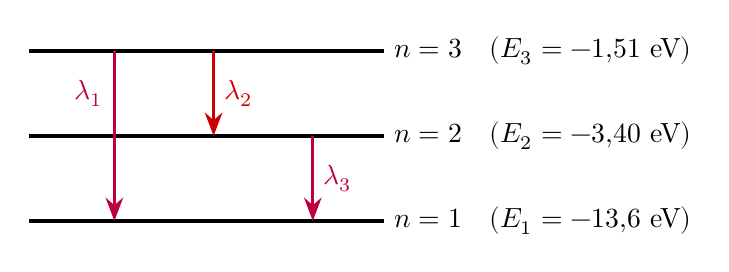
\begin{tikzpicture}[scale=0.9, >=Stealth]
  \draw[very thick] (0, 2.4) -- (5, 2.4) node[right] {$n = 3 \quad (E_3 = -1{,}51\text{ eV})$};
  \draw[very thick] (0, 1.2) -- (5, 1.2) node[right] {$n = 2 \quad (E_2 = -3{,}40\text{ eV})$};
  \draw[very thick] (0, 0) -- (5, 0) node[right] {$n = 1 \quad (E_1 = -13{,}6\text{ eV})$};
  \draw[->, very thick, purple] (1.2, 2.4) -- (1.2, 0) node[pos=0.25, left] {$\lambda_1$};
  \draw[->, very thick, red!80!black] (2.6, 2.4) -- (2.6, 1.2) node[midway, right] {$\lambda_2$};
  \draw[->, very thick, purple] (4.0, 1.2) -- (4.0, 0) node[midway, right] {$\lambda_3$};
\end{tikzpicture}\\[0.1cm]
\textit{Hình 3.1: Các bước dịch chuyển mức năng lượng và vạch phát xạ của nguyên tử Hydro.}
\end{center}

\textbf{B2:} Khi trở về trạng thái cơ bản, nguyên tử phát ra 3 vạch quang phổ tương ứng:
\begin{itemize}[leftmargin=*, topsep=1pt, itemsep=1pt]
  \item Chuyển mức $3 \to 1$:
  \begin{equation*}
      \frac{1}{\lambda_1} = R\left(\frac{1}{1^2} - \frac{1}{3^2}\right) = \frac{8R}{9} \implies \lambda_1 = \frac{9}{8R} = \frac{9}{8 \times 1{,}097 \cdot 10^{-3}} \approx \boldsymbol{1026\text{ \AA}}
  \end{equation*}
  \item Chuyển mức $3 \to 2$ (vạch $H_\alpha$):
  \begin{equation*}
      \frac{1}{\lambda_2} = R\left(\frac{1}{2^2} - \frac{1}{3^2}\right) = \frac{5R}{36} \implies \lambda_2 = \frac{36}{5R} = \frac{36}{5 \times 1{,}097 \cdot 10^{-3}} \approx \boldsymbol{6563\text{ \AA}}
  \end{equation*}
  \item Chuyển mức $2 \to 1$ (vạch $L_\alpha$):
  \begin{equation*}
      \frac{1}{\lambda_3} = R\left(\frac{1}{1^2} - \frac{1}{2^2}\right) = \frac{3R}{4} \implies \lambda_3 = \frac{4}{3R} = \frac{4}{3 \times 1{,}097 \cdot 10^{-3}} \approx \boldsymbol{1215\text{ \AA}}
  \end{equation*}
\end{itemize}

\vspace{0.45cm}

\textbf{Bài 3-4.} Tính mômen từ của một điện tử chuyển động xung quanh một proton trên một quỹ đạo tròn bán kính $r$ (theo vật lý cổ điển).

\textbf{Giải.}

\begin{center}
  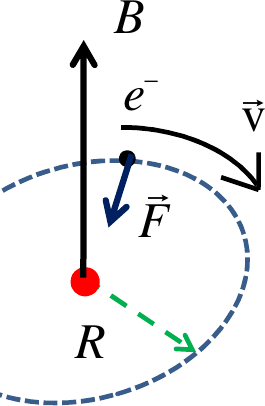
\includegraphics[width=0.28\textwidth]{images/fig_3_4_orbit.png}\\[0.1cm]
  \textit{Hình 3.2: Chuyển động tròn của electron tạo thành dòng điện kín sinh ra mômen từ.}
\end{center}

\textbf{B1:} Cường độ dòng điện tương đương do electron chuyển động tròn chu kỳ $T$ tạo ra:
\begin{equation*}
    I = \frac{e}{T} = \frac{e \omega}{2\pi}
\end{equation*}
Diện tích giới hạn bởi quỹ đạo tròn: $A = \pi r^2$. Mômen từ của nguyên tử:
\begin{equation*}
    |\vec{M}| = I \cdot A = \frac{e \omega}{2\pi} \cdot (\pi r^2) = \frac{1}{2} e \omega r^2
\end{equation*}

\textbf{B2:} AD định luật 2 Newton, lực tĩnh điện Coulomb đóng vai trò lực hướng tâm:
\begin{equation*}
    F_h = \frac{e^2}{4\pi\varepsilon_0 r^2} = m a_n = m \omega^2 r \implies \omega = \sqrt{\frac{e^2}{4\pi\varepsilon_0 m r^3}} = \frac{e}{r}\sqrt{\frac{k}{m r}} \quad \left(k = \frac{1}{4\pi\varepsilon_0}\right)
\end{equation*}

\textbf{B3:} Thay $\omega$ vào biểu thức mômen từ:
\begin{equation*}
    |\vec{M}| = \frac{1}{2} e r^2 \sqrt{\frac{k e^2}{m r^3}} = \boldsymbol{\frac{e^2}{2}\sqrt{\frac{k r}{m}}} = \boldsymbol{\frac{e^2}{2}\sqrt{\frac{r}{4\pi\varepsilon_0 m}}}
\end{equation*}

\vspace{0.45cm}

\textbf{Bài 3-5.} Áp dụng kết quả của cơ học lượng tử tính các giá trị có thể có của mômen từ đối với mức $n = 3$. Biết công thức liên hệ giữa mômen động lượng và mômen từ: $\vec{\mu}_l = -\dfrac{e}{2m}\vec{M}_l$.

\textbf{Giải.}

\textbf{B1:} Với số lượng tử chính $n = 3$, số lượng tử quỹ đạo nhận các giá trị: $l = 0, 1, 2$.
Mômen động lượng quỹ đạo của electron:
\begin{equation*}
    M_l = \hbar \sqrt{l(l+1)}
\end{equation*}
\begin{itemize}[leftmargin=*, topsep=1pt, itemsep=1pt]
  \item $l = 0 \implies M_l = 0$
  \item $l = 1 \implies M_l = \hbar\sqrt{1(2)} = \sqrt{2}\hbar$
  \item $l = 2 \implies M_l = \hbar\sqrt{2(3)} = \sqrt{6}\hbar$
\end{itemize}

\textbf{B2:} Mômen từ quỹ đạo liên hệ qua magneton Bohr $\mu_B = \dfrac{e\hbar}{2m} \approx 9{,}27 \cdot 10^{-24}\text{ J/T}$:
\begin{equation*}
    \mu_l = \frac{e}{2m} M_l = \mu_B \sqrt{l(l+1)}
\end{equation*}
Các giá trị có thể có của mômen từ đối với mức $n = 3$:
\begin{equation*}
    \mu_l = \boldsymbol{0}, \qquad \mu_l = \boldsymbol{\sqrt{2}\mu_B} = \boldsymbol{\frac{e\hbar\sqrt{2}}{2m}}, \qquad \mu_l = \boldsymbol{\sqrt{6}\mu_B} = \boldsymbol{\frac{e\hbar\sqrt{6}}{2m}}
\end{equation*}

\vspace{0.45cm}

\textbf{Bài 3-6.} Biểu diễn các cách định hướng có thể có của mômen động lượng $\vec{M}_l$ với $l = 0, 1, 2, 3$ và $4$ bằng hình vẽ.

\textbf{Giải.}

\textbf{B1:} Định hướng không gian lượng tử hóa:
Hình chiếu của $\vec{M}_l$ lên trục $Oz$ nhận các giá trị gián đoạn $M_{lz} = m_l \hbar$ với số lượng tử từ $m_l = -l, -l+1, \dots, +l$ (tổng cộng $2l + 1$ hướng).
Góc hợp bởi $\vec{M}_l$ và trục $Oz$:
\begin{equation*}
    \cos\varphi = \frac{M_{lz}}{M_l} = \frac{m_l}{\sqrt{l(l+1)}}
\end{equation*}

\begin{center}
  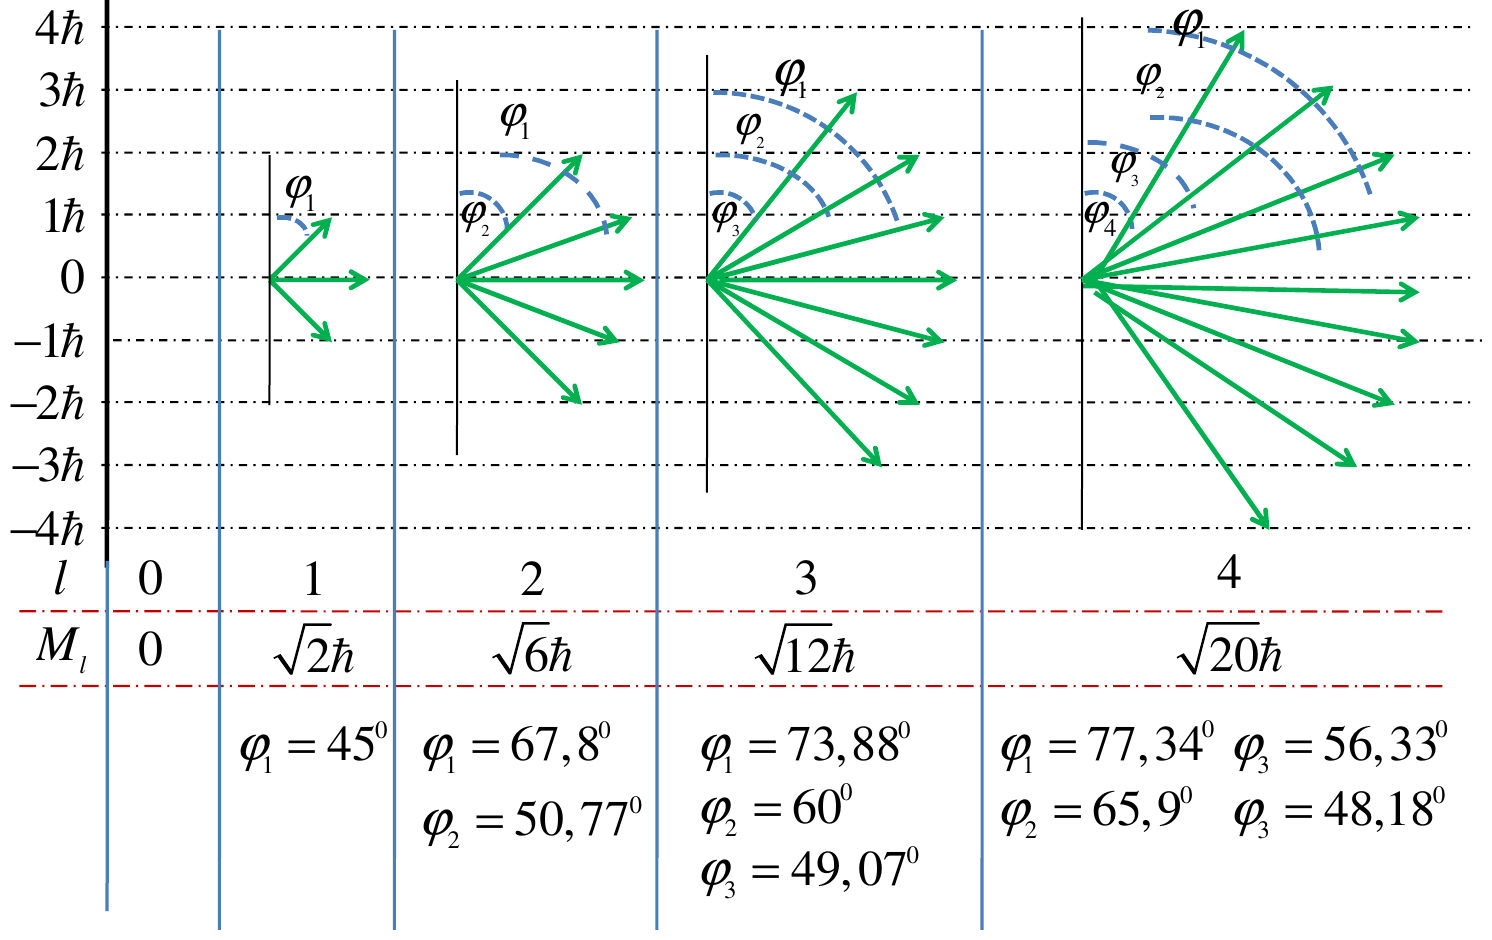
\includegraphics[width=0.92\textwidth]{images/fig_3_6_quantization.png}\\[0.1cm]
  \textit{Hình 3.3: Sự lượng tử hóa không gian của véctơ mômen động lượng quỹ đạo với $l = 0, 1, 2, 3, 4$.}
\end{center}

\vspace{0.45cm}

\textbf{Bài 3-7.} Trong vật lý thiên văn người ta dùng vạch phổ có bước sóng $21\text{ cm}$ để thăm dò vũ trụ. Vạch này được tạo bởi photon phát ra từ nguyên tử hydro của thiên hà khi hướng của spin của điện tử chuyển từ trạng thái song song sang trạng thái phản song song với spin của proton. Tìm giá trị từ trường tác dụng lên điện tử.

\textbf{Giải.}

\textbf{Dữ kiện:} $\lambda = 21\text{ cm} = 0{,}21\text{ m}$, magneton Bohr $\mu_B = \dfrac{e\hbar}{2m} \approx 9{,}27 \cdot 10^{-24}\text{ J/T}$. Cần tìm: $B$.

\textbf{B1:} Năng lượng tương tác giữa mômen từ spin electron và từ trường nội:
\begin{equation*}
    E_B = -\vec{\mu}_s \cdot \vec{B} = \frac{e\hbar}{m} m_s B
\end{equation*}
Khi đảo trạng thái spin từ song song ($m_s = +1/2$) sang đối song ($m_s = -1/2$):
\begin{equation*}
    \Delta E_B = B \frac{e\hbar}{m}\left(\frac{1}{2} - \left(-\frac{1}{2}\right)\right) = B \frac{e\hbar}{m} = 2 \mu_B B
\end{equation*}

\textbf{B2:} Độ chênh lệch năng lượng này phát ra photon bước sóng $\lambda = 21\text{ cm}$:
\begin{equation*}
    \Delta E_B = \frac{h c}{\lambda} \implies 2 \mu_B B = \frac{h c}{\lambda} \implies B = \frac{h c}{2 \mu_B \lambda}
\end{equation*}
Thay số:
\begin{equation*}
    B = \frac{6{,}625 \cdot 10^{-34} \times 3 \cdot 10^8}{2 \times (9{,}27 \cdot 10^{-24}) \times 0{,}21} \approx \boldsymbol{0{,}051\text{ T}} = \boldsymbol{51\text{ mT}}
\end{equation*}

\vspace{0.45cm}

\textbf{Bài 3-8.} Chứng minh rằng các nguyên tử gồm các lớp điền đầy hoàn toàn sẽ có một trạng thái cơ bản $^1S_0$.

\textbf{Giải.}

\textbf{B1:} Khi một phân lớp hoặc lớp electron được điền đầy hoàn toàn:
\begin{itemize}[leftmargin=*, topsep=1pt, itemsep=1pt]
  \item Tổng hình chiếu mômen động lượng quỹ đạo: $M_{Lz} = \sum m_l = 0$. Vì phân lớp đối xứng cầu nên mômen động lượng quỹ đạo toàn phần $L = 0$ (tương ứng ký hiệu quang học trạng thái $S$).
  \item Theo nguyên lý loại trừ Pauli, các trạng thái lượng tử có đủ electron với spin đối song triệt tiêu lẫn nhau: $M_{Sz} = \sum m_s = 0 \implies S = 0$.
\end{itemize}

\textbf{B2:} Độ bội và mômen toàn phần $J$:
\begin{itemize}[leftmargin=*, topsep=1pt, itemsep=1pt]
  \item Độ bội spin: $2S + 1 = 2(0) + 1 = 1$ (trạng thái đơn - singlet).
  \item Mômen động lượng toàn phần: $J = |L - S| = 0$.
\end{itemize}
Kết hợp lại, số hạng phổ của trạng thái cơ bản là $^{2S+1}L_J = \boldsymbol{^1S_0}$ (đpcm).

\vspace{0.5cm}

%=====================================================================
% CHƯƠNG IV
%=====================================================================
\section*{Chương IV. Một số vấn đề vật lý bán dẫn}

\textbf{Bài 4-1.} Nồng độ hạt dẫn trong bán dẫn riêng thay đổi như thế nào khi nhiệt độ chất bán dẫn thay đổi từ $200\text{ K}$ đến $300\text{ K}$ và bề rộng vùng cấm giả thiết thay đổi theo quy luật $\Delta E_g(T) = (0{,}785 - \alpha T)\text{ eV}$.

\textbf{Giải.}

\textbf{Dữ kiện:} $T_1 = 200\text{ K}$, $T_2 = 300\text{ K}$, $\Delta E_g(T) = \Delta E_g(0) - \alpha T$ với $\Delta E_g(0) = 0{,}785\text{ eV}$.

\textbf{B1:} Nồng độ hạt dẫn trong bán dẫn riêng:
\begin{equation*}
    n_i(T) = \sqrt{N_c N_v} e^{-\Delta E_g(T)/(2kT)}
\end{equation*}
Mật độ trạng thái hiệu dụng phụ thuộc nhiệt độ: $N_c \propto T^{3/2}, N_v \propto T^{3/2} \implies \sqrt{N_c N_v} \propto T^{3/2}$.

\textbf{B2:} Thay quy luật $\Delta E_g(T) = \Delta E_g(0) - \alpha T$:
\begin{equation*}
    \exp\left(-\frac{\Delta E_g(0) - \alpha T}{2kT}\right) = \exp\left(\frac{\alpha}{2k}\right) \exp\left(-\frac{\Delta E_g(0)}{2kT}\right)
\end{equation*}
Tỉ số nồng độ hạt dẫn riêng tại hai nhiệt độ:
\begin{equation*}
    \frac{n_i(300\text{ K})}{n_i(200\text{ K})} = \left(\frac{300}{200}\right)^{3/2} \exp\left[-\frac{\Delta E_g(0)}{2k}\left(\frac{1}{300} - \frac{1}{200}\right)\right] = \left(\frac{3}{2}\right)^{3/2} \exp\left[\frac{\Delta E_g(0)}{2k} \cdot \frac{100}{60000}\right]
\end{equation*}
Thay số với $\Delta E_g(0) = 0{,}785\text{ eV}$ và $k = 8{,}617 \cdot 10^{-5}\text{ eV/K}$:
\begin{equation*}
    \frac{\Delta E_g(0)}{2k \times 600} = \frac{0{,}785}{2 \times 8{,}617 \cdot 10^{-5} \times 600} = \frac{0{,}785}{0{,}1034} \approx 7{,}59
\end{equation*}
\begin{equation*}
    \frac{n_i(300\text{ K})}{n_i(200\text{ K})} = (1{,}5)^{1{,}5} \times e^{7{,}59} \approx 1{,}837 \times 1978 \approx \boldsymbol{3{,}6 \cdot 10^3}
\end{equation*}
Nồng độ hạt dẫn riêng tăng xấp xỉ $\boldsymbol{3600\text{ lần}}$.

\vspace{0.45cm}

\textbf{Bài 4-3.} Tính nồng độ điện tử, lỗ trống, vị trí mức Fermi (so với đỉnh vùng hóa trị) của silic chứa $1{,}1 \cdot 10^{16}\text{ nguyên tử B trên } 1\text{ cm}^3$ ở nhiệt độ $300\text{ K}$. Các đại lượng trên sẽ thay đổi như thế nào khi pha thêm vào mẫu các nguyên tử photpho với nồng độ $9 \cdot 10^{15}\text{ nguyên tử P trên } 1\text{ cm}^3$.

\textbf{Giải.}

\textbf{Dữ kiện:} $N_c = 2{,}8 \cdot 10^{19}\text{ cm}^{-3}$, $N_v = 1 \cdot 10^{19}\text{ cm}^{-3}$, $n_i = 1{,}45 \cdot 10^{10}\text{ cm}^{-3}$, $kT = 0{,}026\text{ eV}$ ở $300\text{ K}$.

\textbf{B1:} Mẫu Silic ban đầu chứa Bo ($N_a = 1{,}1 \cdot 10^{16}\text{ cm}^{-3}$):
Vì Bo là tạp chất nhóm III (acceptor) nên đây là bán dẫn loại p không suy biến:
\begin{itemize}[leftmargin=*, topsep=1pt, itemsep=1pt]
  \item Nồng độ lỗ trống: $p_0 \approx N_a = \boldsymbol{1{,}1 \cdot 10^{16}\text{ cm}^{-3}}$.
  \item Nồng độ electron:
  \begin{equation*}
      n_0 = \frac{n_i^2}{p_0} = \frac{(1{,}45 \cdot 10^{10})^2}{1{,}1 \cdot 10^{16}} \approx \boldsymbol{1{,}91 \cdot 10^4\text{ cm}^{-3}}
  \end{equation*}
  \item Vị trí mức Fermi so với đỉnh vùng hóa trị $E_v$:
  \begin{equation*}
      E_f = E_v + kT \ln\left(\frac{N_v}{N_a}\right) = E_v + 0{,}026 \ln\left(\frac{10^{19}}{1{,}1 \cdot 10^{16}}\right) \approx \boldsymbol{E_v + 0{,}177\text{ eV}}
  \end{equation*}
\end{itemize}

\textbf{B2:} Sau khi pha thêm Photpho ($N_d = 9 \cdot 10^{15}\text{ cm}^{-3}$):
Photpho là tạp chất nhóm V (donor). Vì $N_a > N_d$ nên mẫu vẫn là bán dẫn loại p bị bù trừ:
\begin{itemize}[leftmargin=*, topsep=1pt, itemsep=1pt]
  \item Nồng độ lỗ trống mới:
  \begin{equation*}
      p_0' = N_a - N_d = 1{,}1 \cdot 10^{16} - 9 \cdot 10^{15} = \boldsymbol{2 \cdot 10^{15}\text{ cm}^{-3}}
  \end{equation*}
  \item Nồng độ electron mới:
  \begin{equation*}
      n_0' = \frac{n_i^2}{p_0'} = \frac{(1{,}45 \cdot 10^{10})^2}{2 \cdot 10^{15}} \approx \boldsymbol{1{,}05 \cdot 10^5\text{ cm}^{-3}} \approx \boldsymbol{1 \cdot 10^5\text{ cm}^{-3}}
  \end{equation*}
  \item Vị trí mức Fermi mới:
  \begin{equation*}
      E_f' = E_v + kT \ln\left(\frac{N_v}{N_a - N_d}\right) = E_v + 0{,}026 \ln\left(\frac{10^{19}}{2 \cdot 10^{15}}\right) \approx \boldsymbol{E_v + 0{,}277\text{ eV}}
  \end{equation*}
\end{itemize}

\vspace{0.45cm}

\textbf{Bài 4-4.} Hãy chứng minh công thức nồng độ điện tử trong bán dẫn suy biến loại $n$:
\begin{equation*}
    n = \frac{8\pi}{3}\left(\frac{2m_n^*}{h^2}\right)^{3/2}(E_f - E_c)^{3/2}
\end{equation*}

\textbf{Giải.}

\textbf{B1:} Trong tinh thể, electron dẫn được xem như tự do với khối lượng hiệu dụng $m_n^*$. Theo nguyên lý bất định Heisenberg đối với không gian 3 chiều:
\begin{equation*}
    \Delta p_x \Delta x \ge h, \quad \Delta p_y \Delta y \ge h, \quad \Delta p_z \Delta z \ge h \implies \Delta V_p = \Delta p_x \Delta p_y \Delta p_z \ge \frac{h^3}{V}
\end{equation*}
Trong thể tích $V = 1$ đơn vị, mỗi trạng thái lượng tử chiếm một ô thể tích $h^3$ trong không gian xung lượng $\vec{p}$. Mỗi trạng thái lượng tử chứa tối đa 2 electron có spin đối song.

\textbf{B2:} Ở nhiệt độ thấp ($T \to 0\text{ K}$), trong bán dẫn suy biến loại n, tất cả các mức năng lượng từ đáy vùng dẫn $E_c$ đến mức Fermi $E_f$ bị điền đầy hoàn toàn. Trong không gian xung lượng, các electron chiếm đầy một hình cầu Fermi bán kính $p_F$:
\begin{equation*}
    \frac{p_F^2}{2m_n^*} = E_f - E_c \implies p_F = \sqrt{2m_n^*(E_f - E_c)}
\end{equation*}
Thể tích hình cầu Fermi đó là:
\begin{equation*}
    V_{pF} = \frac{4\pi}{3} p_F^3 = \frac{4\pi}{3} \left[2m_n^*(E_f - E_c)\right]^{3/2}
\end{equation*}

\textbf{B3:} Số electron trên một đơn vị thể tích bán dẫn:
\begin{equation*}
    n = 2 \cdot \frac{V_{pF}}{h^3} = 2 \cdot \frac{\dfrac{4\pi}{3} \left[2m_n^*(E_f - E_c)\right]^{3/2}}{h^3} = \boldsymbol{\frac{8\pi}{3}\left(\frac{2m_n^*}{h^2}\right)^{3/2}(E_f - E_c)^{3/2}}
\end{equation*}
Đây chính là hệ thức cần chứng minh.

\vspace{0.45cm}

\textbf{Bài 4-5.} Giả sử bán dẫn Si loại $n^+$ với $N_d = 10^{17}\text{ cm}^{-3}$ tiếp xúc với Si loại $n$ với $N_d = 10^{14}\text{ cm}^{-3}$ (hoặc Si loại $p$ với $N_a = 10^{14}\text{ cm}^{-3}$). Hãy tính mức Fermi trong từng vật liệu và vẽ sơ đồ vùng năng lượng tiếp xúc.

\textbf{Giải.}

\textbf{Dữ kiện:} $N_c = 2{,}8 \cdot 10^{19}\text{ cm}^{-3}$, $N_v = 10^{19}\text{ cm}^{-3}$, $\Delta E_g = 1{,}12\text{ eV}$, $kT = 0{,}026\text{ eV}$.

\textbf{B1:} Xác định mức Fermi trong từng vật liệu riêng biệt:
\begin{itemize}[leftmargin=*, topsep=1pt, itemsep=1pt]
  \item Vật liệu thứ nhất (loại $n^+$, $N_{d1} = 10^{17}\text{ cm}^{-3}$):
  \begin{equation*}
      E_{f1} = E_c - kT \ln\left(\frac{N_c}{N_{d1}}\right) = E_c - 0{,}026 \ln\left(\frac{2{,}8 \cdot 10^{19}}{10^{17}}\right) = \boldsymbol{E_c - 0{,}1465\text{ eV}}
  \end{equation*}
  \item Vật liệu thứ hai (loại $n$, $N_{d2} = 10^{14}\text{ cm}^{-3}$):
  \begin{equation*}
      E_{f2} = E_c - kT \ln\left(\frac{N_c}{N_{d2}}\right) = E_c - 0{,}026 \ln\left(\frac{2{,}8 \cdot 10^{19}}{10^{14}}\right) = \boldsymbol{E_c - 0{,}326\text{ eV}}
  \end{equation*}
  \item Vật liệu thứ ba (loại $p$, $N_{a3} = 10^{14}\text{ cm}^{-3}$):
  \begin{equation*}
      E_{f3} = E_v + kT \ln\left(\frac{N_v}{N_{a3}}\right) = E_v + 0{,}026 \ln\left(\frac{10^{19}}{10^{14}}\right) = \boldsymbol{E_v + 0{,}299\text{ eV}} = \boldsymbol{E_c - 0{,}821\text{ eV}}
  \end{equation*}
\end{itemize}

\begin{center}
  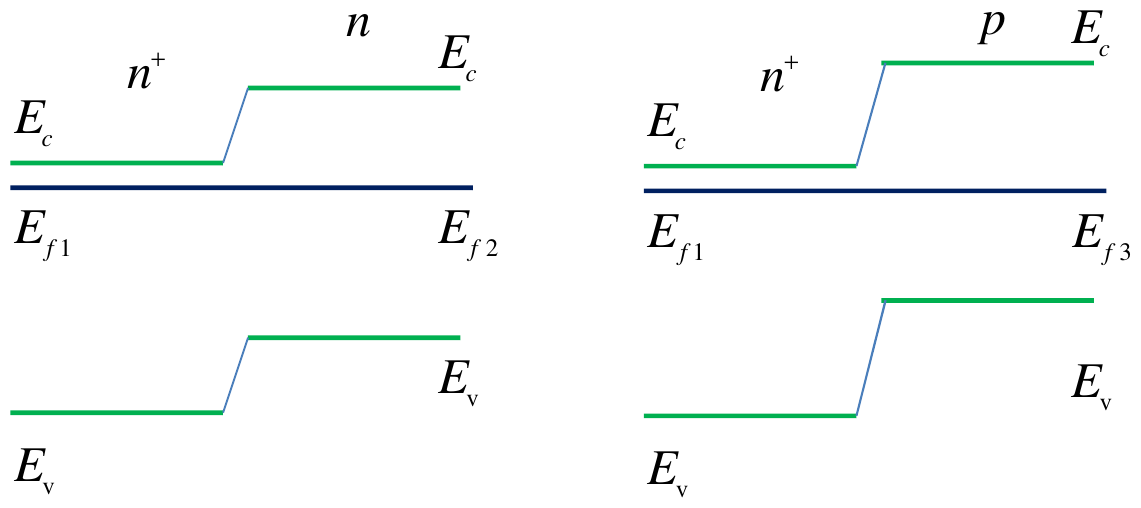
\includegraphics[width=0.72\textwidth]{images/fig_4_5_band_diagram.png}\\[0.1cm]
  \textit{Hình 4.1: Sơ đồ vùng năng lượng tiếp xúc $n^+ - n$ và tiếp xúc $n^+ - p$ ở trạng thái cân bằng.}
\end{center}

\vspace{0.45cm}

\textbf{Bài 4-6.} Tính độ dẫn của silic tinh khiết ở $300\text{ K}$. Biết $n_i = 1{,}45 \cdot 10^{10}\text{ cm}^{-3}$, $\mu_n = 1450\text{ cm}^2/\text{V}\cdot\text{s}$, $\mu_p = 450\text{ cm}^2/\text{V}\cdot\text{s}$. Tính độ dẫn khi pha tạp $N_d = 10^{14}\text{ cm}^{-3}$ và $N_a = 10^{17}\text{ cm}^{-3}$.

\textbf{Giải.}

\textbf{B1:} Độ dẫn của Si tinh khiết:
\begin{equation*}
    \sigma_i = e n_i (\mu_n + \mu_p) = 1{,}6 \cdot 10^{-19} \times 1{,}45 \cdot 10^{10} \times (1450 + 450) \approx \boldsymbol{4{,}4 \cdot 10^{-6}\text{ }\Omega^{-1}\text{cm}^{-1}}
\end{equation*}
Điện trở suất: $\rho_i = \dfrac{1}{\sigma_i} \approx \boldsymbol{22{,}7 \cdot 10^4\text{ }\Omega\cdot\text{cm}}$.

\textbf{B2:} Khi pha tạp donor $N_d = 10^{14}\text{ cm}^{-3}$ ($n_0 \approx N_d \gg p_0$):
\begin{equation*}
    \sigma_n \approx e N_d \mu_n = 1{,}6 \cdot 10^{-19} \times 10^{14} \times 1450 = \boldsymbol{2{,}32 \cdot 10^{-2}\text{ }\Omega^{-1}\text{cm}^{-1}}
\end{equation*}
Điện trở suất: $\rho_n = \dfrac{1}{\sigma_n} \approx \boldsymbol{43{,}1\text{ }\Omega\cdot\text{cm}}$.

\textbf{B3:} Khi pha tạp acceptor $N_a = 10^{17}\text{ cm}^{-3}$ ($p_0 \approx N_a \gg n_0$):
\begin{equation*}
    \sigma_p \approx e N_a \mu_p = 1{,}6 \cdot 10^{-19} \times 10^{17} \times 450 = \boldsymbol{7{,}2\text{ }\Omega^{-1}\text{cm}^{-1}}
\end{equation*}
Điện trở suất: $\rho_p = \dfrac{1}{\sigma_p} \approx \boldsymbol{0{,}139\text{ }\Omega\cdot\text{cm}}$.

\vspace{0.45cm}

\textbf{Bài 4-7.} Tính hiệu công thoát điện tử giữa hai mẫu silic, mẫu thứ nhất pha tạp loại $n$ với $N_d = 1 \cdot 10^{15}\text{ cm}^{-3}$, mẫu thứ hai pha tạp loại $p$ với $N_a = 1 \cdot 10^{17}\text{ cm}^{-3}$ (hoặc $10^{15}\text{ cm}^{-3}$). Cho biết $\Delta E_g = 1{,}12\text{ eV}$, $kT = 0{,}026\text{ eV}$, $N_c = 2{,}8 \cdot 10^{19}\text{ cm}^{-3}$, $N_v = 1 \cdot 10^{19}\text{ cm}^{-3}$.

\textbf{Giải.}

\textbf{B1:} Mức Fermi trong từng mẫu so với bờ vùng:
\begin{itemize}[leftmargin=*, topsep=1pt, itemsep=1pt]
  \item Mẫu 1 (loại $n$):
  \begin{equation*}
      E_{f1} = E_c - kT \ln\left(\frac{N_c}{N_d}\right) = E_c - 0{,}026 \ln\left(\frac{2{,}8 \cdot 10^{19}}{10^{15}}\right) \approx \boldsymbol{E_c - 0{,}266\text{ eV}}
  \end{equation*}
  \item Mẫu 2 (loại $p$ với $N_a = 10^{17}\text{ cm}^{-3}$):
  \begin{equation*}
      E_{f2} = E_v + kT \ln\left(\frac{N_v}{N_a}\right) = E_v + 0{,}026 \ln\left(\frac{10^{19}}{10^{17}}\right) \approx \boldsymbol{E_v + 0{,}119\text{ eV}}
  \end{equation*}
\end{itemize}

\textbf{B2:} Hiệu công thoát $\Delta\Phi$ và điện thế tiếp xúc $U_k$:
Vì công thoát $\Phi = E_0 - E_f$ (với $E_0$ là mức chân không):
\begin{equation*}
    \Delta\Phi = \Phi_2 - \Phi_1 = E_{f1} - E_{f2} = (E_c - 0{,}266) - (E_v + 0{,}119) = \Delta E_g - 0{,}385\text{ eV}
\end{equation*}
\begin{equation*}
    \Delta\Phi = 1{,}12\text{ eV} - 0{,}385\text{ eV} = \boldsymbol{0{,}735\text{ eV}} \implies U_k = \boldsymbol{0{,}735\text{ V}}
\end{equation*}

\vspace{0.5cm}

%=====================================================================
% CHƯƠNG V
%=====================================================================
\section*{Chương V. Xử lý tín hiệu quang -- Quang điện tử}

\textbf{Bài 5-1.} Chứng minh công thức tính khẩu độ số ($NA$ -- Numerical Aperture) của sợi quang:
\begin{equation*}
    NA = \sin\theta_{i,\max} = \sqrt{n_1^2 - n_2^2} \approx n_1 \sqrt{2\Delta}
\end{equation*}
trong đó $n_1, n_2$ là chiết suất của lõi và vỏ; $\Delta = \dfrac{n_1 - n_2}{n_1}$ là độ chênh chiết suất tương đối.

\textbf{Giải.}

\begin{center}
  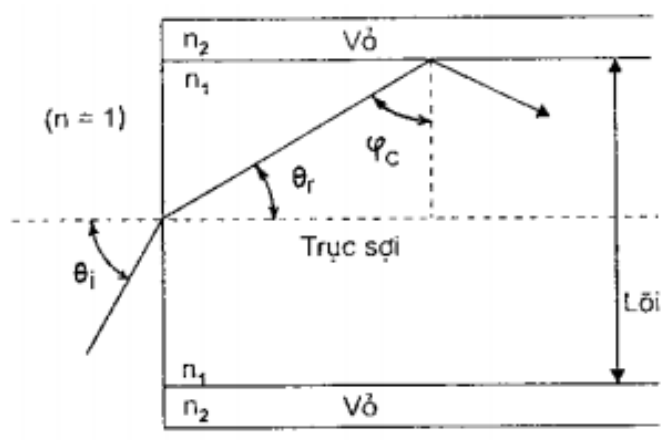
\includegraphics[width=0.55\textwidth]{images/fig_5_1_fiber_na.png}\\[0.1cm]
  \textit{Hình 5.1: Đường truyền tia sáng và điều kiện phản xạ toàn phần trong sợi quang.}
\end{center}

\textbf{B1:} AD định luật khúc xạ tại mặt đầu sợi quang (từ không khí $n_0 = 1$ vào lõi chiết suất $n_1$):
\begin{equation*}
    \sin\theta_i = n_1 \sin\theta_r
\end{equation*}
Từ hình học tam giác vuông tại mặt phân cách lõi -- vỏ: $\theta_r + \varphi_c = 90^\circ \implies \sin\theta_r = \cos\varphi_c$.
\begin{equation*}
    \implies \sin\theta_i = n_1 \cos\varphi_c
\end{equation*}

\textbf{B2:} Điều kiện để tia sáng truyền dẫn được trong sợi quang là phải xảy ra phản xạ toàn phần tại mặt biên lõi -- vỏ:
\begin{equation*}
    \sin\varphi_c \ge \frac{n_2}{n_1}
\end{equation*}
Khi góc tới mặt đầu lớn nhất ($\theta_{i,\max}$), góc phản xạ ở mặt biên đạt giá trị tới hạn $\sin\varphi_c = \dfrac{n_2}{n_1}$:
\begin{equation*}
    \cos\varphi_c = \sqrt{1 - \sin^2\varphi_c} = \sqrt{1 - \frac{n_2^2}{n_1^2}} = \frac{\sqrt{n_1^2 - n_2^2}}{n_1}
\end{equation*}

\textbf{B3:} Thay vào biểu thức của $\sin\theta_{i,\max}$:
\begin{equation*}
    NA = \sin\theta_{i,\max} = n_1 \cos\varphi_c = \boldsymbol{\sqrt{n_1^2 - n_2^2}}
\end{equation*}
Mặt khác: $n_1^2 - n_2^2 = (n_1 - n_2)(n_1 + n_2) \approx (n_1\Delta)(2n_1) = 2 n_1^2 \Delta$. Do đó:
\begin{equation*}
    NA \approx \boldsymbol{n_1 \sqrt{2\Delta}}
\end{equation*}
Đây chính là hệ thức cần chứng minh.

\vspace{0.45cm}

\textbf{Bài 5-2.} Từ điều kiện các mode dẫn truyền trong sợi quang giật cấp đa mode, bỏ qua sự dịch chuyển pha do phản xạ ở mặt phân cách lõi -- vỏ, đánh giá số lượng các mode đó cho $d = 10\lambda_0$, $n_1 = 1{,}5$, độ chênh chiết suất $\Delta = 0{,}02$.

\textbf{Giải.}

\textbf{Dữ kiện:} $d = 10\lambda_0$, $n_1 = 1{,}5$, $\Delta = 0{,}02$.

\begin{center}
  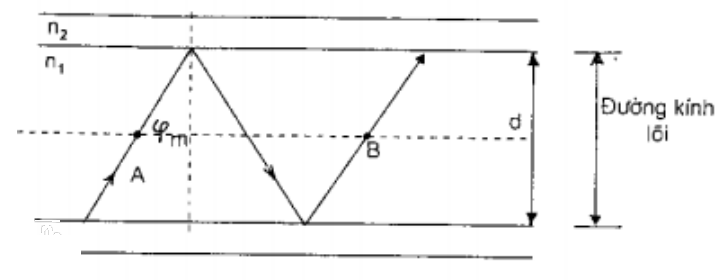
\includegraphics[width=0.55\textwidth]{images/fig_5_2_fiber_modes.png}\\[0.1cm]
  \textit{Hình 5.2: Phản xạ zigzag của mode dẫn truyền trong sợi quang phẳng.}
\end{center}

\textbf{B1:} Điều kiện dẫn truyền mode sóng trong sợi quang:
\begin{itemize}[leftmargin=*, topsep=1pt, itemsep=1pt]
  \item ĐK phản xạ toàn phần: $\sin\varphi_m \ge \dfrac{n_2}{n_1}$.
  \item ĐK can nhiễu đồng pha sau hai lần phản xạ liên tiếp:
  \begin{equation*}
      d \sin\theta_c \ge m \frac{\lambda}{2} = m \frac{\lambda_0}{2 n_1}, \qquad (m = 0, 1, 2, \dots, N-1)
  \end{equation*}
\end{itemize}

\textbf{B2:} Mode bậc cao nhất ứng với góc tới hạn $\sin\theta_c = \sin\theta_{i,\max}/n_1 \approx \sqrt{2\Delta}$:
\begin{equation*}
    N \le \frac{2 d}{\lambda_0} n_1 \sin\theta_c = \frac{2 d}{\lambda_0} n_1 \sqrt{2\Delta}
\end{equation*}
Thay số:
\begin{equation*}
    N \le 2 \times 10 \times 1{,}5 \times \sqrt{2 \times 0{,}02} = 30 \times \sqrt{0{,}04} = 30 \times 0{,}2 = \boldsymbol{6\text{ mode}}
\end{equation*}

\vspace{0.45cm}

\textbf{Bài 5-4.} Cho một bán dẫn vùng cấm thẳng tinh khiết có bề rộng vùng cấm $\Delta E_g = 1{,}5\text{ eV}$, giả sử khối lượng hiệu dụng của điện tử và lỗ trống là đẳng hướng, bằng nhau và bằng $\frac{m_0}{10} = 9{,}1 \cdot 10^{-32}\text{ kg}$.
\begin{enumerate}[label=\alph*)]
  \item Tính bước sóng ngưỡng hấp thụ quang học riêng.
  \item Khi chiếu sáng mạnh làm nồng độ hạt dẫn tăng cao, ngưỡng hấp thụ thay đổi như thế nào? (Hiệu ứng Burstein-Moss).
\end{enumerate}

\textbf{Giải.}

\textbf{B1:} Bước sóng ngưỡng hấp thụ của bán dẫn tinh khiết ban đầu:
\begin{equation*}
    \lambda_{th} = \frac{h c}{\Delta E_g} = \frac{1{,}24}{\Delta E_g\text{ (eV)}}\text{ }\mu\text{m} = \frac{1{,}24}{1{,}5} \approx \boldsymbol{0{,}827\text{ }\mu\text{m}}
\end{equation*}

\textbf{B2:} Khi chiếu sáng mạnh, mật độ electron quang sinh trong vùng dẫn và lỗ trống trong vùng hóa trị tăng rất cao. Theo nguyên lý loại trừ Pauli, các trạng thái năng lượng thấp ở đáy vùng dẫn bị lấp đầy tới mức cận Fermi $E_{fn}^*$, và đỉnh vùng hóa trị bị lấp đầy tới mức $E_{fp}^*$.

Photon tới chỉ có thể kích thích electron từ trạng thái hóa trị chưa bị chiếm lên trạng thái dẫn còn trống. Điều kiện hấp thụ dịch chuyển vùng cấm quang học:
\begin{equation*}
    h\nu \ge \Delta E_g + \Delta E_n + \Delta E_p
\end{equation*}
Do đó ngưỡng năng lượng hấp thụ tăng lên, tương ứng bước sóng ngưỡng quang học bị \textbf{dịch về phía sóng ngắn} (hiệu ứng Burstein-Moss): $\lambda_{th}' \approx \boldsymbol{0{,}788\text{ }\mu\text{m}}$.

\vspace{0.45cm}

\textbf{Bài 5-5.} Một mẫu bán dẫn đơn tinh thể silic có bề dày $0{,}25\text{ }\mu\text{m}$ được chiếu sáng bằng ánh sáng đơn sắc có $h\nu = 3\text{ eV}$ với công suất $10\text{ mW}$. Tìm năng lượng tổng cộng mà mẫu hấp thụ trong $1$ giây, năng lượng nhiệt truyền cho mạng tinh thể trong $1\text{ s}$ và số photon sinh ra do tái hợp bức xạ riêng (vùng -- vùng). Cho hệ số hấp thụ $\alpha = 4 \cdot 10^4\text{ cm}^{-1}$, $\Delta E_g = 1{,}12\text{ eV}$.

\textbf{Giải.}

\textbf{Dữ kiện:} $d = 0{,}25\text{ }\mu\text{m} = 0{,}25 \cdot 10^{-4}\text{ cm}$, $P_0 = 10\text{ mW} = 10^{-2}\text{ W}$, $h\nu = 3\text{ eV}$, $\Delta E_g = 1{,}12\text{ eV}$, $\alpha = 4 \cdot 10^4\text{ cm}^{-1}$.

\textbf{B1:} Năng lượng ánh sáng bị mẫu hấp thụ trong thời gian $1\text{ s}$:
\begin{equation*}
    \Delta\Phi = P_0 (1 - e^{-\alpha d}) = 10^{-2} \times \left[1 - \exp(-4 \cdot 10^4 \times 0{,}25 \cdot 10^{-4})\right] = 10^{-2}(1 - e^{-1}) \approx \boldsymbol{6{,}32 \cdot 10^{-3}\text{ J}}
\end{equation*}
(Công suất hấp thụ tương ứng là $\boldsymbol{6{,}3\text{ mW}}$).

\textbf{B2:} Năng lượng nhiệt truyền cho mạng tinh thể trong $1\text{ s}$:
Mỗi photon hấp thụ giải phóng một cặp điện tử -- lỗ trống có dư năng lượng $h\nu - \Delta E_g$. Năng lượng dư này nhanh chóng hồi phục nhiệt truyền cho dao động mạng tinh thể (phonon):
\begin{equation*}
    \eta_T = \frac{h\nu - \Delta E_g}{h\nu} = \frac{3 - 1{,}12}{3} = \frac{1{,}88}{3} \approx 62{,}67\%
\end{equation*}
Năng lượng nhiệt truyền cho mạng trong $1\text{ s}$:
\begin{equation*}
    Q_T = \Delta\Phi \times \eta_T = 6{,}32 \cdot 10^{-3} \times 62{,}67\% \approx \boldsymbol{3{,}9 \cdot 10^{-3}\text{ J}} = \boldsymbol{3{,}9\text{ mJ}}
\end{equation*}

\textbf{B3:} Năng lượng tái hợp bức xạ riêng và số photon phát ra:
\begin{itemize}[leftmargin=*, topsep=1pt, itemsep=1pt]
  \item Năng lượng bức xạ tái hợp trong $1\text{ s}$:
  \begin{equation*}
      Q_{\text{rad}} = \Delta\Phi - Q_T = 6{,}32 \cdot 10^{-3} - 3{,}96 \cdot 10^{-3} \approx \boldsymbol{2{,}4 \cdot 10^{-3}\text{ J}}
  \end{equation*}
  \item Mỗi photon tái hợp vùng -- vùng mang năng lượng $\Delta E_g = 1{,}12\text{ eV} = 1{,}12 \times 1{,}6 \cdot 10^{-19}\text{ J}$:
  \begin{equation*}
      N_{\text{photon}} = \frac{Q_{\text{rad}}}{\Delta E_g} = \frac{2{,}4 \cdot 10^{-3}}{1{,}12 \times 1{,}6 \cdot 10^{-19}} \approx \boldsymbol{1{,}3 \cdot 10^{16}\text{ photon/s}}
  \end{equation*}
\end{itemize}

\vspace{0.45cm}

\textbf{Bài 5-6.} Một mẫu GaAs được chiếu sáng bởi ánh sáng có bước sóng $\lambda = 0{,}6\text{ }\mu\text{m}$. Công suất tia tới là $15\text{ mW}$. Nếu $1/3$ công suất đó bị phản xạ trở lại và $1/3$ thoát ra từ mặt sau của mẫu thì bề dày của mẫu bằng bao nhiêu? Tìm năng lượng nhiệt được truyền cho mạng tinh thể trong một giây. Biết hệ số hấp thụ $\alpha(0{,}6\text{ }\mu\text{m}) = 5 \cdot 10^4\text{ cm}^{-1}$, $\Delta E_g = 1{,}42\text{ eV}$.

\textbf{Giải.}

\textbf{Dữ kiện:} $\lambda = 0{,}6\text{ }\mu\text{m}$, $P_0 = 15\text{ mW}$, $P_{\text{phản xạ}} = \dfrac{1}{3} P_0$, $P_{\text{thoát}} = \dfrac{1}{3} P_0$, $\alpha = 5 \cdot 10^4\text{ cm}^{-1}$, $\Delta E_g = 1{,}42\text{ eV}$.

\textbf{B1:} Xác định bề dày mẫu $d$:
Công suất truyền vào trong mẫu sau khi phản xạ bề mặt trước: $P_1 = P_0 (1 - R) = P_0\left(1 - \dfrac{1}{3}\right) = \dfrac{2}{3}P_0$.
Công suất thoát ra ở mặt sau:
\begin{equation*}
    P_{\text{thoát}} = P_1 e^{-\alpha d} = \frac{2}{3} P_0 e^{-\alpha d}
\end{equation*}
Theo đề bài, $P_{\text{thoát}} = \dfrac{1}{3} P_0$, suy ra:
\begin{equation*}
    \frac{2}{3} P_0 e^{-\alpha d} = \frac{1}{3} P_0 \implies 2 e^{-\alpha d} = 1 \implies e^{\alpha d} = 2 \implies d = \frac{\ln 2}{\alpha}
\end{equation*}
Thay số:
\begin{equation*}
    d = \frac{0{,}6931}{5 \cdot 10^4\text{ cm}^{-1}} \approx 1{,}386 \cdot 10^{-5}\text{ cm} = \boldsymbol{0{,}139\text{ }\mu\text{m}}
\end{equation*}

\textbf{B2:} Năng lượng nhiệt truyền cho mạng tinh thể trong $1\text{ s}$:
\begin{itemize}[leftmargin=*, topsep=1pt, itemsep=1pt]
  \item Năng lượng photon tới: $h\nu = \dfrac{h c}{\lambda} = \dfrac{1{,}24}{0{,}6} \approx 2{,}067\text{ eV}$.
  \item Phần trăm năng lượng nhiệt truyền cho mạng tinh thể từ mỗi photon:
  \begin{equation*}
      \eta_T = \frac{h\nu - \Delta E_g}{h\nu} = \frac{2{,}067 - 1{,}42}{2{,}067} = \frac{0{,}647}{2{,}067} \approx 31{,}3\%
  \end{equation*}
  \item Công suất ánh sáng hấp thụ thực tế trong mẫu:
  \begin{equation*}
      P_{\text{hấp thụ}} = P_1 - P_{\text{thoát}} = \frac{2}{3} P_0 - \frac{1}{3} P_0 = \frac{1}{3} P_0 = \frac{15\text{ mW}}{3} = 5\text{ mW}
  \end{equation*}
  \item Năng lượng nhiệt truyền cho mạng tinh thể trong $1\text{ s}$:
  \begin{equation*}
      Q_T = P_{\text{hấp thụ}} \times \eta_T = 5\text{ mW} \times 31{,}3\% \approx \boldsymbol{1{,}56\text{ mW}} = \boldsymbol{1{,}56 \cdot 10^{-3}\text{ J}}
  \end{equation*}
\end{itemize}

\vspace{0.45cm}

\textbf{Bài 5-7.} Một quang dẫn có kích thước $L = 6\text{ mm}$, $W = 2\text{ mm}$, $D = 1\text{ mm}$ được chiếu bởi bức xạ đồng đều. Do hấp thụ ánh sáng dòng điện tăng lên $2{,}83\text{ mA}$. Điện áp đặt lên $2$ cực là $10\text{ V}$. Khi ngắt nguồn sáng đột ngột dòng điện giảm với vận tốc ban đầu là $23{,}6\text{ A/s}$. Cho biết $\mu_n = 3600\text{ cm}^2/\text{V}\cdot\text{s}$, $\mu_p = 1700\text{ cm}^2/\text{V}\cdot\text{s}$.
\begin{enumerate}[label=\alph*)]
  \item Tính nồng độ hạt dẫn dư dừng.
  \item Tính thời gian sống của các hạt dẫn.
  \item Tìm nồng độ hạt dẫn sau khi ngắt nguồn sáng một khoảng thời gian $t = 10^{-3}\text{ s}$.
\end{enumerate}

\textbf{Giải.}

\textbf{Dữ kiện:} $L = 6\text{ mm} = 6 \cdot 10^{-3}\text{ m}$, $W = 2\text{ mm} = 2 \cdot 10^{-3}\text{ m}$, $D = 1\text{ mm} = 10^{-3}\text{ m}$, $U = 10\text{ V}$, $\Delta I = 2{,}83\text{ mA} = 2{,}83 \cdot 10^{-3}\text{ A}$, $\left|\dfrac{dI}{dt}\right|_{t=0} = 23{,}6\text{ A/s}$, $\mu_n = 3600\text{ cm}^2/\text{V}\cdot\text{s} = 0{,}36\text{ m}^2/\text{V}\cdot\text{s}$, $\mu_p = 1700\text{ cm}^2/\text{V}\cdot\text{s} = 0{,}17\text{ m}^2/\text{V}\cdot\text{s}$.

\textbf{B1:} Nồng độ hạt dẫn dư dừng $n_{st}$:
Mật độ dòng điện quang dẫn:
\begin{equation*}
    J = \sigma E = e n_{st}(\mu_n + \mu_p) \frac{U}{L}
\end{equation*}
Dòng điện qua tiết diện $S = W \cdot D$:
\begin{equation*}
    \Delta I = J \cdot S = e n_{st}(\mu_n + \mu_p) \frac{U}{L} (W \cdot D)
\end{equation*}
Suy ra nồng độ hạt dẫn dư dừng:
\begin{equation*}
    n_{st} = \frac{\Delta I \cdot L}{e (\mu_n + \mu_p) U W D}
\end{equation*}
Thay số:
\begin{align*}
    n_{st} &= \frac{2{,}83 \cdot 10^{-3} \times 6 \cdot 10^{-3}}{1{,}6 \cdot 10^{-19} \times (0{,}36 + 0{,}17) \times 10 \times (2 \cdot 10^{-3} \times 10^{-3})} \\
    &= \frac{1{,}698 \cdot 10^{-5}}{1{,}696 \cdot 10^{-24}} \approx \boldsymbol{10^{19}\text{ m}^{-3}} = \boldsymbol{10^{13}\text{ cm}^{-3}}
\end{align*}

\textbf{B2:} Thời gian sống của hạt dẫn $\tau$:
Sau khi ngắt nguồn sáng, dòng điện giảm theo quy luật hàm mũ:
\begin{equation*}
    I(t) = I_0 e^{-t/\tau} \implies \left.\frac{dI}{dt}\right|_{t=0} = -\frac{I_0}{\tau} \implies \tau = \frac{I_0}{\left|\dfrac{dI}{dt}\right|_{t=0}}
\end{equation*}
Thay số với $I_0 = 2{,}83 \cdot 10^{-3}\text{ A}$ và tốc độ giảm ban đầu $23{,}6\text{ A/s}$:
\begin{equation*}
    \tau = \frac{2{,}83 \cdot 10^{-3}}{23{,}6} \approx \boldsymbol{0{,}12 \cdot 10^{-3}\text{ s}} = \boldsymbol{0{,}12\text{ ms}}
\end{equation*}

\textbf{B3:} Nồng độ hạt dẫn sau khi ngắt nguồn sáng $t = 10^{-3}\text{ s}$:
\begin{align*}
    n(t) &= n_{st} e^{-t/\tau} = 10^{13} \times \exp\left(-\frac{10^{-3}}{0{,}12 \cdot 10^{-3}}\right) \\
    &= 10^{13} \times e^{-8{,}333} \approx 10^{13} \times 2{,}40 \cdot 10^{-4} \approx \boldsymbol{2{,}4 \cdot 10^9\text{ cm}^{-3}}
\end{align*}

\end{document}
